\documentclass[english]{iamthesis}
% changle "slovak" to "english" for english version of the thesis

%----------------------------------------------------------------%
% THESIS DATA

% thesis level {bc | ing | min | dis}
\def\thesislevel{bc}

% student name with title e.g. Ing. Martin Klaučo
\def\thesisauthor{Ivana Dukayová} 

% year of submmiting to AIS
\def\thesisyear{2024}

% registration number generated by AIS e.g. 19990-50920
\def\thesisnumber{číslo práce} 

% thesis type: BACHELOR|MASTER|DISSERTATION or in slovak 
% BAKALÁRSKA|DIPLOMOVÁ|DIZERTAČNÁ
\def\thesistype{BACHELOR}

% thesis title
\def\thesistitle{Touchless Drone Control}

% thesis supervisor including degrees e.g. Ing. Martin Klaučo, PhD.
\def\thesissupervisor{Ing. Martin Klaučo, PhD.}

% study field (translate to english if neccesarry) e.g. "Riadenie Procesov" or
% "Process Control"
\def\thesisprogram{Process Control}

% Institute (translate to english if neccesary)
% e.g., "Institute of Information Engineering, Automation, and Mathematics"
\def\thesisinst{Institute of Information Engineering, Automation, and Mathematics}

% Title of the Acknowledgment
% For slovak write: "Poďakovanie" for English write: "Acknowledgment"
\def\thesisack{Acknowledgment}


% End THESIS DATA
%----------------------------------------------------------------%

%----------------------------------------------------------------%
%   Titles and other stuff                                       %
%----------------------------------------------------------------%
\author{\thesisauthor}
\title{\thesistitle}
\date{\today}
%\usepackage{layouts}
%\usepackage{layout}
\usepackage{hyperref}
%\usepackage[margin=1cm]{geometry}
\usepackage{tikz,pgfplots,pgf}
\usetikzlibrary{arrows.meta} % <-- Make sure this line is here
\usepackage{tikz-qtree}
\usetikzlibrary{matrix,shapes,arrows,positioning}
%----------------------------------------------------------------%
%   Let the document begin                                       %
%----------------------------------------------------------------%
\begin{document}

% ---------------------------------------------------------------%
% The Frontmatter  !! Do NOT change the structure !!             % 
%----------------------------------------------------------------%

\coverpage

\frontmatter
\pagenumbering{roman}

% include assignment generated by AIS system
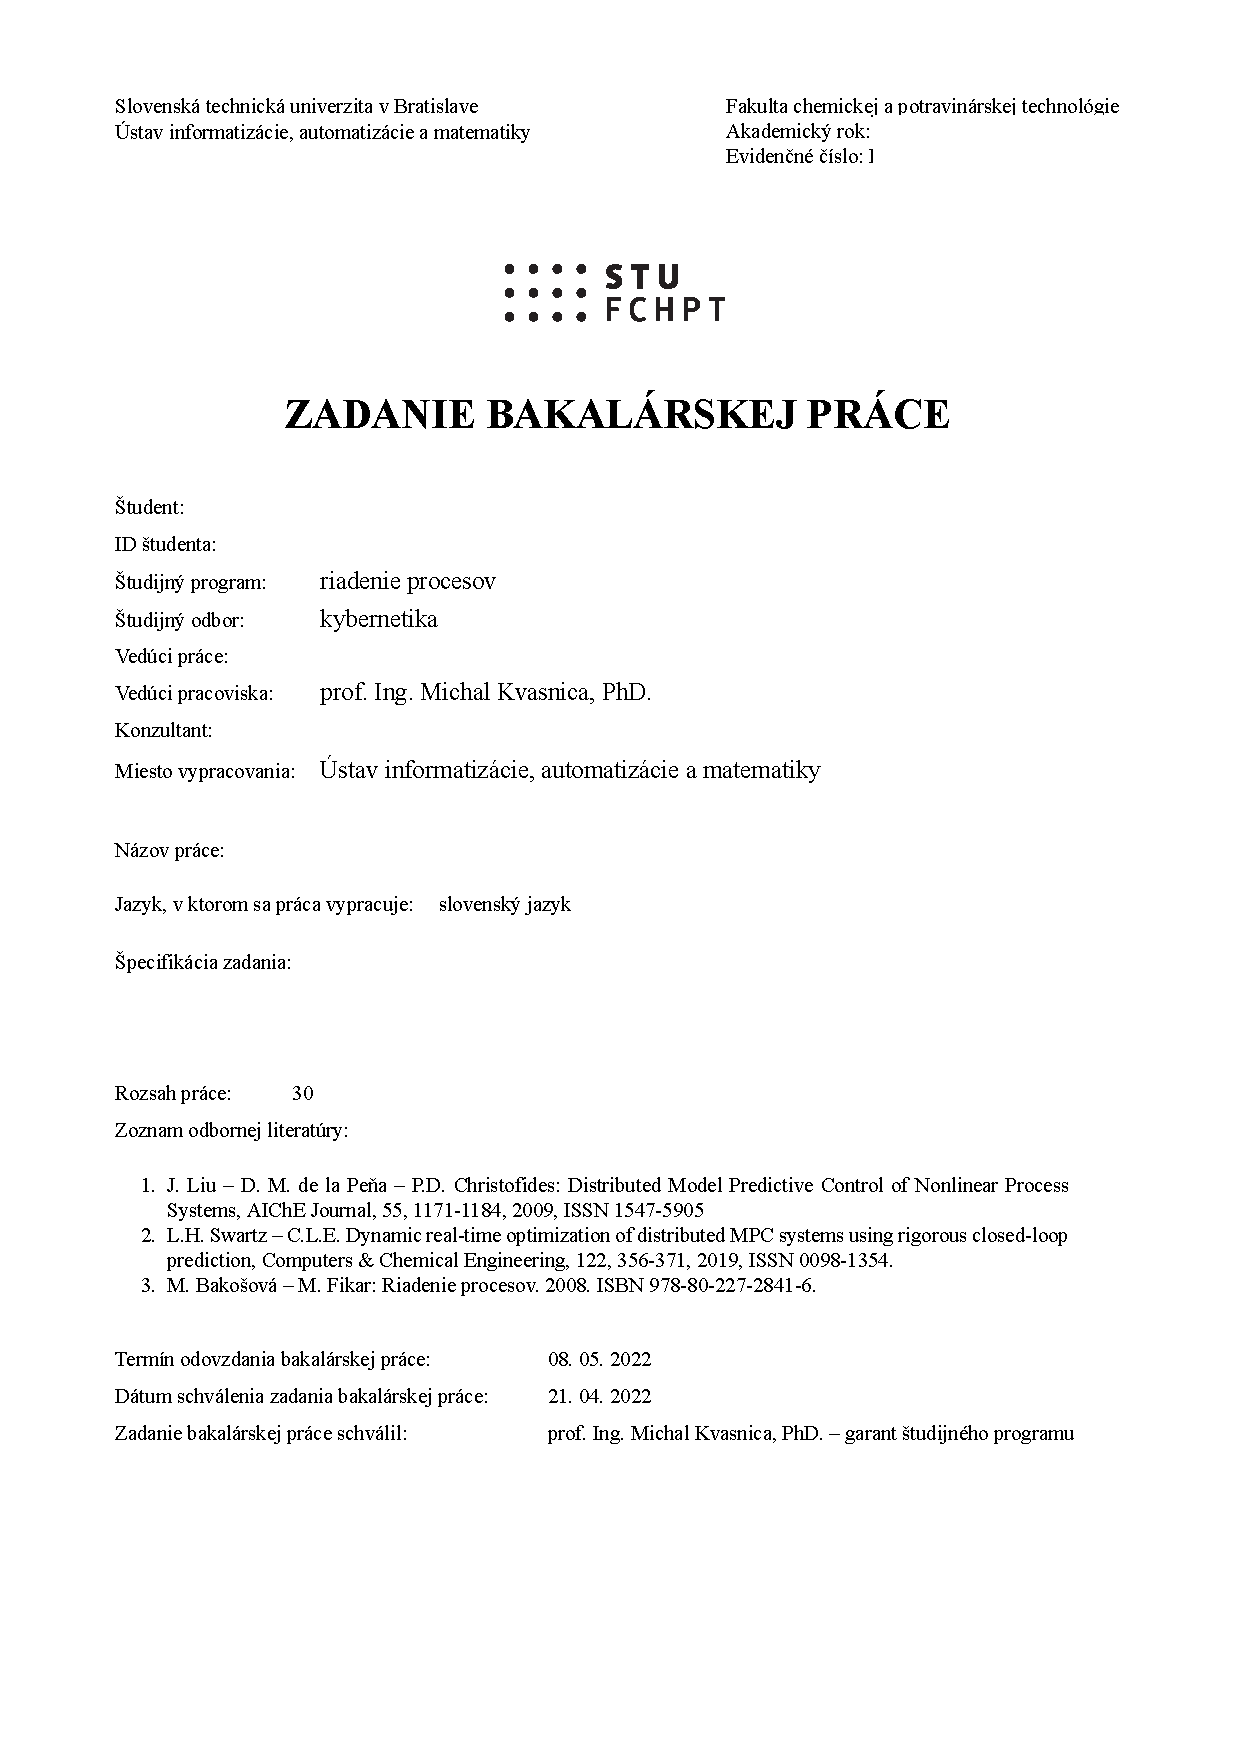
\includepdf[pages=-]{content/zadanie.pdf}
% use this command only if your assignment has more than 2 pages
% 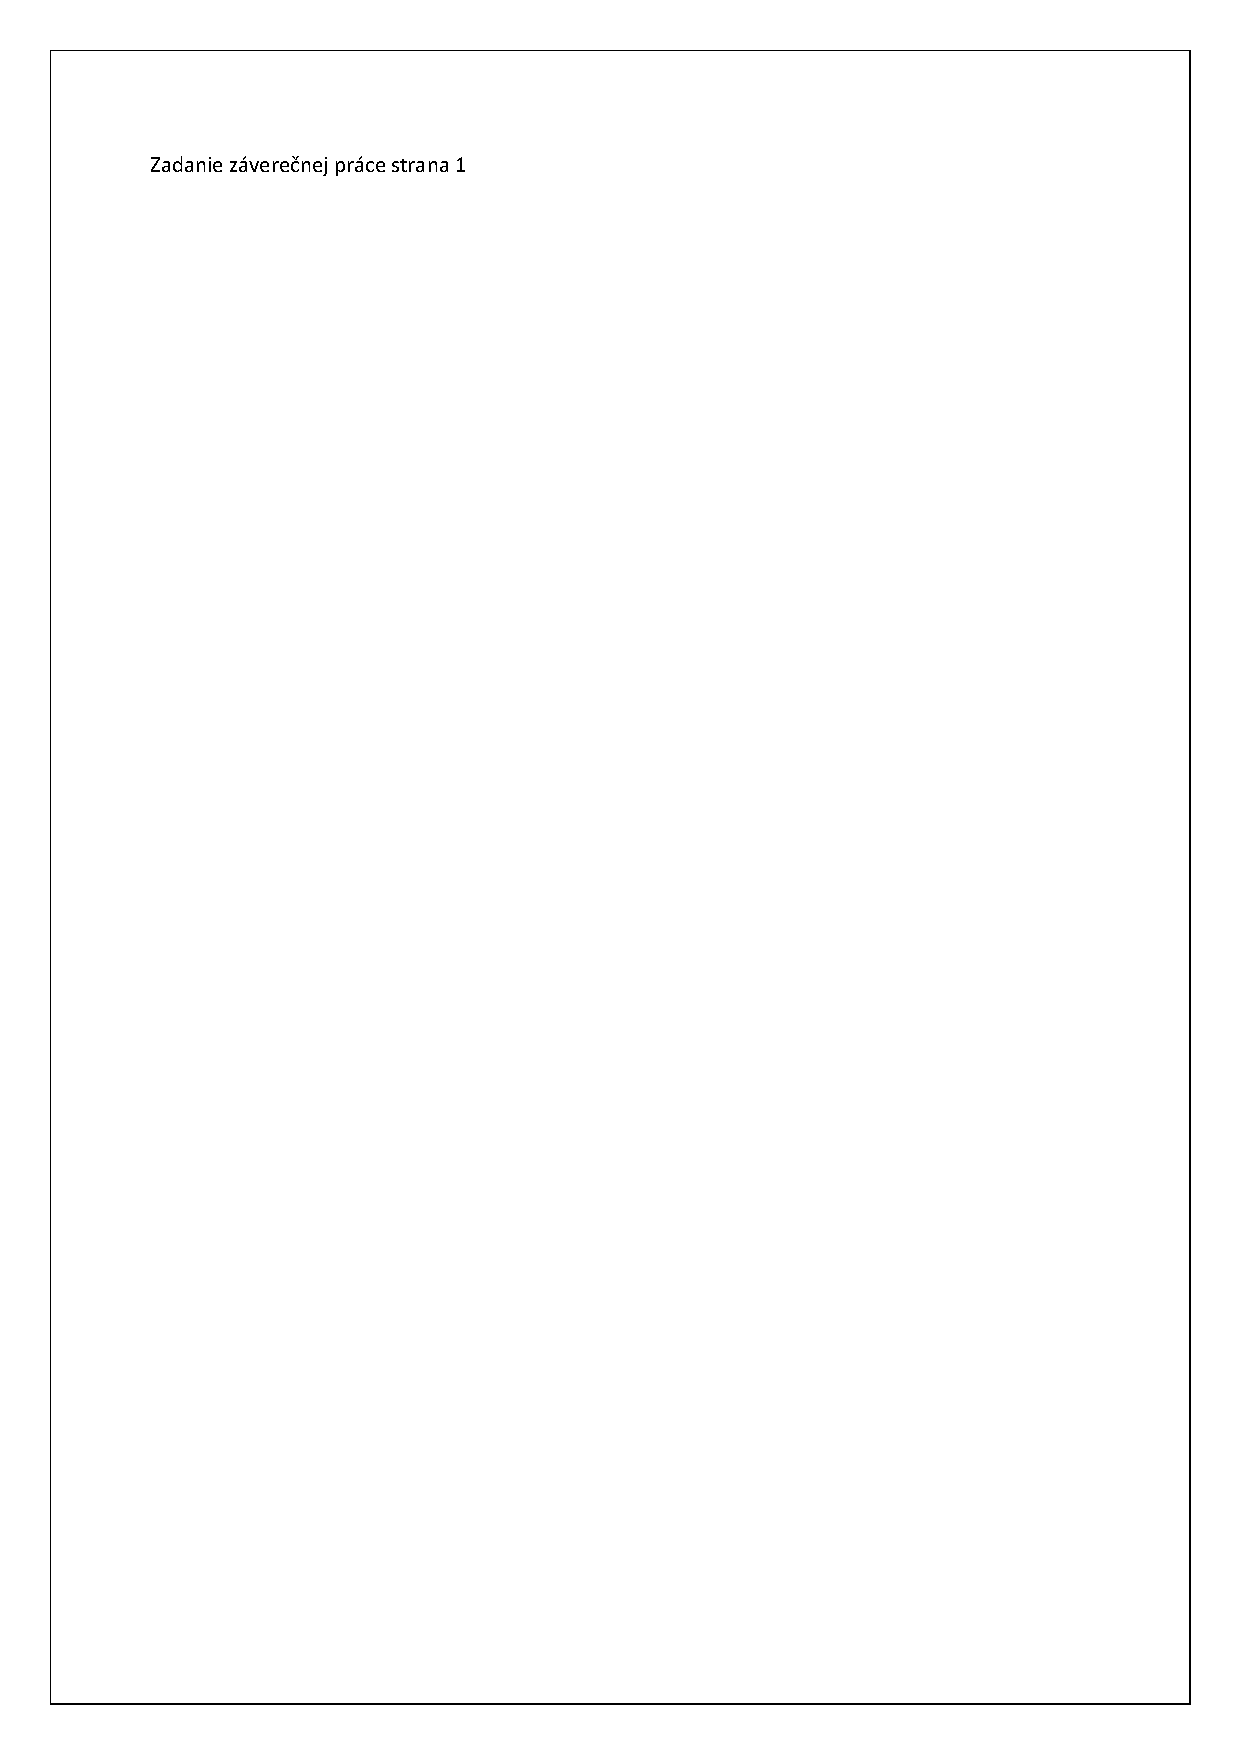
\includepdf[page=2]{content/assignment.pdf}


% do not remove following commands
% do not following commands
\chapter*{\thesisack}
\markboth{}{}
\addcontentsline{toc}{chapter}{\thesisack}
I am deeply grateful to Ing. Patrik Valabek for his insightful advice while we worked on this project, reminding me there is no turning back now. His guidance was crucial in dealing with these changes and helped me navigate the challenges and opportunities.
Special thanks also to my supervisor, doc. Ing. MSc. Martin Klaučo, PhD., for his guidance, patience, and feedback throughout my thesis journey. 
I appreciate the encouragement from my peers, who provided the encouragement needed to harness the madness of our journey, particularly in moments when the world is a scary place.
Lastly, thanks to all my friends and family, for the times I found myself looking at my own reflection to recognize that something profound is slowly changing in me.

\chapter*{Abstract}
\markboth{}{}
\addcontentsline{toc}{chapter}{Abstract}
% English abstract
This project focuses on identifying gestures using a drone's camera and controlling the drone based on these gestures. Our target area is to create a reliable system for gesture recognition and drone control without the need for creating complex mathematical models.

Our work includes using the drone's camera to capture gestures and identifying these gestures using the MediaPipe library. We aim to recognize various gestures, including those that control drone movements such as ascents, descents, rotations, and taking photographs. For identification, we have implemented a neural network model that we trained on the collected dataset containing various hand gestures. In conjunction with the OpenCV library for image processing, the model is capable of recognizing and classifying gestures in real-time based on footage from the drone's camera.

Our work has enabled us to successfully identify various gestures and control the drone based on these recognized gestures. The project also demonstrates how gesture recognition can be a practical and interesting method for interacting with drones, allowing people to intuitively control these devices.

\chapter*{Abstrakt}
\markboth{}{}
\addcontentsline{toc}{chapter}{Abstrakt}
% Slovenský abstrakt

\setcounter{tocdepth}{2}
\renewcommand{\baselinestretch}{0.1}\normalsize
\tableofcontents

\listoffigures
\listoftables

\renewcommand{\baselinestretch}{1.1}\normalsize

% ----------------------------------------------------------------%
% The Mainmatter !! Do NOT change the structure!!                 %
% ----------------------------------------------------------------%
\mainmatter

% individual chapters should be included via a separate tex file, as shown in 
% here. When working in TexStudio (recomennded tool for Win and Mac) set the 
% main.tex as an Explicit root document, so you can compile even you are
% working on other chapter in other tex file.
%
% Open main.tex THEN click Options-> Root Document -> Set Current Document as
% Explicit Root

% introduction
\clearpage
\chapter{Introduction}
\label{ch:intro}

As robots continue to become more integrated into our daily lives, researchers are working to improve human-robot interaction. Gesture recognition technology has emerged as a key tool for enabling more natural interactions with robots, replacing traditional human-machine interfaces like keyboards, mice, and joysticks. This application can be a good intervention for people with disabilities. By using hand gestures, they can more easily interact with virtual environments, robotics, home automation, clinical operations, game controls, desktop/tablet applications, delivery services, sign language, and more. 
Drones are remotely controlled robots can be operated via a remote control device or smartphone. They're a popular tool in many of these applications, often used for sports event coverage, aerial photography, and emergency response. Developing automatic systems that can recognize hand gestures would greatly improve the ability to interact with drones intuitively.
\\ Our goal is to create a real-time hand gesture recognition system for human-drone interaction. In this project, we have achieved touchless interaction between the drone and our hands. We utilized machine learning technology, specifically MediaPipe, for hand tracking and developed a gesture recognition model that underwent rigorous training and testing. The process involves five steps: 
\begin{enumerate}[label=\Roman*.]
	\item Drone capturing an image
	\item Image processing via OpenCV
	\item Gesture recognition
	\item Gesture - command conversion
	\item Command execution
	
\end{enumerate}
Gesture recognition is used in various sectors, including smart home automation and the medical field. It mainly focuses on human-machine interaction. The system receives input images from a drone camera connected to the device. The main goal of this project is to propose a real-time system with high accuracy. In summary, the project demonstrates how we can control a drone in an entertaining and educational way while highlighting the potential of gesture recognition technology in various industries and applications.
\begin{figure}
	\centering
	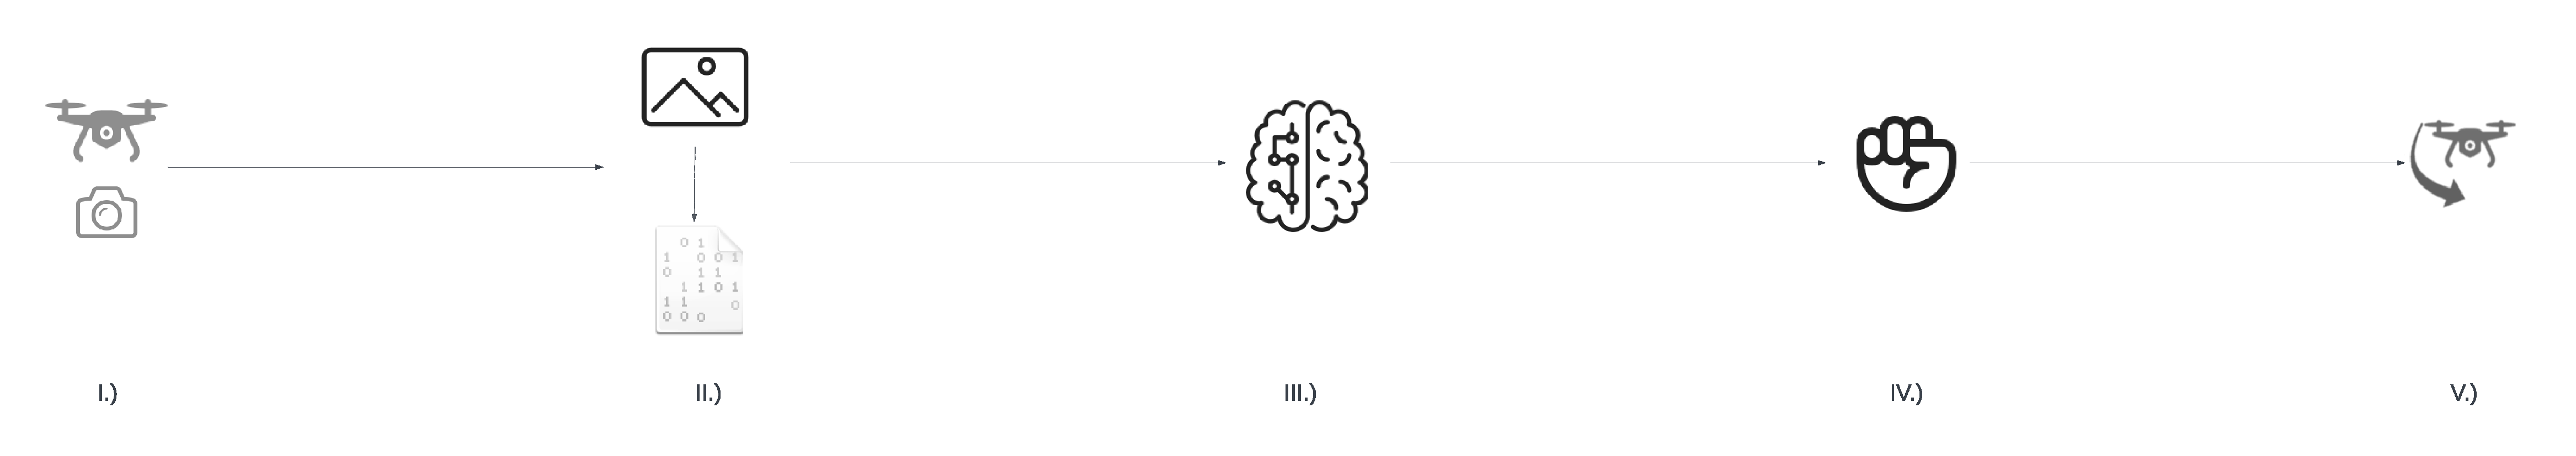
\includegraphics[width = \textwidth]{images/steps.pdf}
	\caption{Steps of the process}
	\label{fig:conclusion}
\end{figure}


% theory
\chapter{Theory}


\section{Machine Learning}
Machine learning, or ML for short, is a branch of artificial intelligence (AI) that focuses on creating computer algorithms that learn automatically from data and experience. It allows computers to learn from data and make predictions or decisions without the need for explicit programming.
With the rapid advancement of AI, machines are now able to solve complex problems with greater ease. Learning methods can be broadly classified into two main categories - supervised learning and unsupervised learning. In addition to these, there are other methods such as reinforcement learning, semi-supervised learning, and many hybrid approaches.

Supervised learning involves training a computer algorithm with input data that has been labeled for a specific output. To enable it to produce accurate labeling results when presented with never-before-seen data, the model is trained until it can identify the underlying patterns and relationships between the input data and the output labels. Making sense of the data for a particular question is the goal of supervised learning. Classification and regression problems are well-suited for supervised learning. 


With classification, one of a known number of categories is represented by the output variable. For instance, "dog" or "cat," "positive" or "negative." Popular techniques used for classification involve a logistic regression, a decision tree, a random forest, or a support vector machine.


The regression's value of the output variable is continuous or actual. For instance, "geographical location", and "price". The following algorithms are frequently employed: linear regression, nonlinear regression, a regression tree, or Bayesian logic.


Unsupervised learning relies on an unlabeled dataset for training, without requiring any correct output values as in supervised learning. Instead, the algorithm identifies patterns and similarities within the data, independent of external measurements. This approach allows algorithms to explore and uncover unexpected insights that may not have been anticipated by humans.

Two more problem categories for the unsupervised learning algorithm are clustering and association.


With clustering, objects are grouped into clusters, so that those with the greatest similarities stay in that group and have little to no similarities with other objects in the group.


An association rule is used to determine the relationships between variables in a large database. An association rule improves the efficacy of marketing strategy. For example, consumers who purchase X (bread, for example) also frequently buy Y (butter).


Some of the popular unsupervised learning algorithms include K-means clustering, KNN, hierarchal clustering, or anomaly detection.

\section{Techniques used in Computer Vision }
In Computer Vision (CV), ML plays an important role in extracting important information from images. CV successfully contributes to various domains, surveillance systems, optical character recognition, robotics, suspect detection, and many more.  The direction of CV research is going towards the healthcare domain, medical imaging (MI) is an emerging technology, that plays a vital role in improving image quality and recognizing critical features of binary medical images, covert original images into grayscale, and set the threshold for segmentation.
Within computer vision, three key tasks stand out: segmentation, detection, and classification.
\subsection*{Image Classifiaction}
It's a known fact that the image we see as a whole is made up of hundreds to thousands of tiny pixels. Before computer vision can determine and label the image as a whole, it needs to analyze the individual components of the image. That is why image classification techniques analyze a given image in the form of pixels and accomplish this by treating the picture as an array of matrices, the size of which is determined by the image resolution. The pixels of the digital image are taken and grouped into what we know as “classes.” From this point on, the procedure will vary depending on the algorithm. To guarantee that it is not left entirely on the final classifier, the selected algorithm will convert the image into a series of key attributes. These characteristics aid the classifier in identifying the subject matter and class to which the image belongs.
We can say that the image classification pipeline looks like this:
image pre-processing -> feature extraction -> object classification


Based on the nature of the problem, there are different types of image classification methodologies. They are binary, multiclass, multilabel, and hierarchical.

Binary classification divides unknown data points into two groups using an either-or logic for labeling images. Binary classification is used to handle many different yes/no problems, such as analyzing product quality to determine whether a product has faults, and many more tasks requiring judgment calls.

As the name implies, multiclass divides objects into three or more classes, whereas binary classification divides objects into two classes. It's highly helpful in a variety of fields, including medical diagnostics (disease categorization), NLP (sentiment analysis in situations involving several emotions), etc.

The multilabel method permits an object to be allocated to more than one label, in contrast to multiclass classification, which assigns an image to a single class. For instance, you could have to categorize multiple colors in an image. Taking a picture of a salad, a picture of one will feature red, orange, yellow, purple, and other colors. Consequently, several colors will be used as labels on a single image.

The process of classifying classes into a hierarchical structure based on their similarities is known as hierarchical classification. A lower-level class is more definite and detailed, while a higher-level class represents larger categories. If we're classifying a dog, our first model would recognize a dog vs another animal. If a dog is correctly predicted, another model will be used to classify the breed of the dog into border collie, golden retriever, and poodle. All features of higher-class attributes will be hierarchically contained in the latter ones. Hierarchy allows for effective information transfer between related classes as well as a flexible and interpretable framework for organizing and representing complex visual concepts.


Image Classification correlates one class from the training data with a whole image or video frame regardless of the amount of information present. It involves assigning labels and is suitable when fine-grained information is not necessary. During the model training stage, publically accessible datasets are frequently employed to enable correct data labeling.
\subsection*{Object Detection}
The classification is advanced in object detection. It not only classifies many objects in an image but also provides annotations for the bounding boxes that correspond to each entity's position. The CV model's extra benefits enable its implementation in several practical contexts as these models are only a small portion of detecting, labeling, and annotating objects in images or videos. Faster R-CNN \cite{girshick2014rich}, YOLO (You Only Look Once) \cite{redmon2016you}, and SSD (Single Shot MultiBox Detector)\cite{liu2016ssd} are a few popular object detection algorithms. These algorithms are tailored to specific application requirements and differ in terms of speed, accuracy, and trade-offs.  An example of an object detection model is a model for human detection. The model would return a bounding box around each person with a label

\begin{figure}[ht]
	\centering
	\begin{minipage}{0.4\textwidth}
		\centering
		
\includegraphics[width=0.7\linewidth]{images/cat_class.jpg}
		\caption*{Cat}
		\label{fig:justcat}
	\end{minipage}% <-- Add this percentage sign here
	\begin{minipage}{0.48\textwidth}
		\centering
		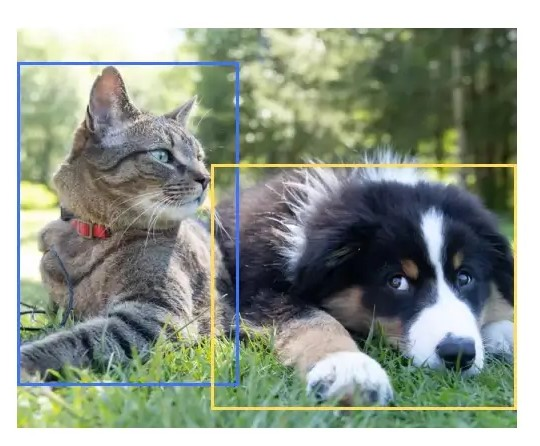
\includegraphics[width=0.7\linewidth]{images/catanddog_detect.jpg}
		\caption*{Cat, Dog}
		\label{fig:catanddog}
	\end{minipage}
	\caption{Comparison of classification (left) with output: 'Cat' and object detection (right) with output: 'Cat, Dog' and their localization with bounding boxes }
	\label{fig:both_figures_class_detect} % This label can now be used to reference both images together
\end{figure}



\subsection*{Image Segmentation}

Since they both serve the same purpose, object detection and image segmentation are comparable. Both techniques identify items in pictures and provide coordinates for locating objects. However, segmentation algorithms produce accurate masks that cover objects at the pixel level, as opposed to creating whole boxes around them.

Annotations for image segmentation include the exact pixel locations of any instances that are present in the image. Image segmentation is better suitable for practical uses because of its accurate results. However, compared to object detection, picture segmentation models are computationally expensive due to algorithm complexity.
The example used is in applying visual effects like background blurring and makeup effects to the image. The functionality identifies specific textures, colors, and segments of object features within image data. It is also widely used in medical imaging, self-driving cars, or satellite imaging.

In figure \ref{fig:segmentation} a U-Net \cite{ronneberger2015u}, an architecture introduced by Olaf Ronneberger, Philipp Fischer, and Thomas Brox in 2015 is used. It's a convolutional neural network that was specifically designed to be used in Biomedical Imaging. A pre-trained model MobileNetV2 \cite{sandler2018mobilenetv2} is used as a lightweight, efficient feature extractor for the input image. It would analyze the photo of the dog and create a set of feature maps highlighting important visual attributes like edges, textures, and shapes relevant to the segmentation task. Then, with the feature maps provided by MobileNetV2, U-Net would take on the task of image segmentation. Its architecture, designed to work with fewer data points and to be precise in delineating object boundaries, would use the feature maps to generate a predicted mask. It would attempt to closely replicate the true mask by classifying each pixel as belonging to the dog or the background. A Pix2Pix \cite{isola2017image} model is then used to generate a segmented image that tries to match the true mask, learning the mapping from the input image to the segmentation mask during training.

For this task, it is also possible to use interactive segmentation, which divides the image into two regions: the selected object and everything else. It receives a location in an image, calculates the object's boundaries at that location, and returns image data that defines the object's area.



\begin{figure}[ht]
	\centering
	\begin{minipage}{0.3\textwidth}
		\centering
		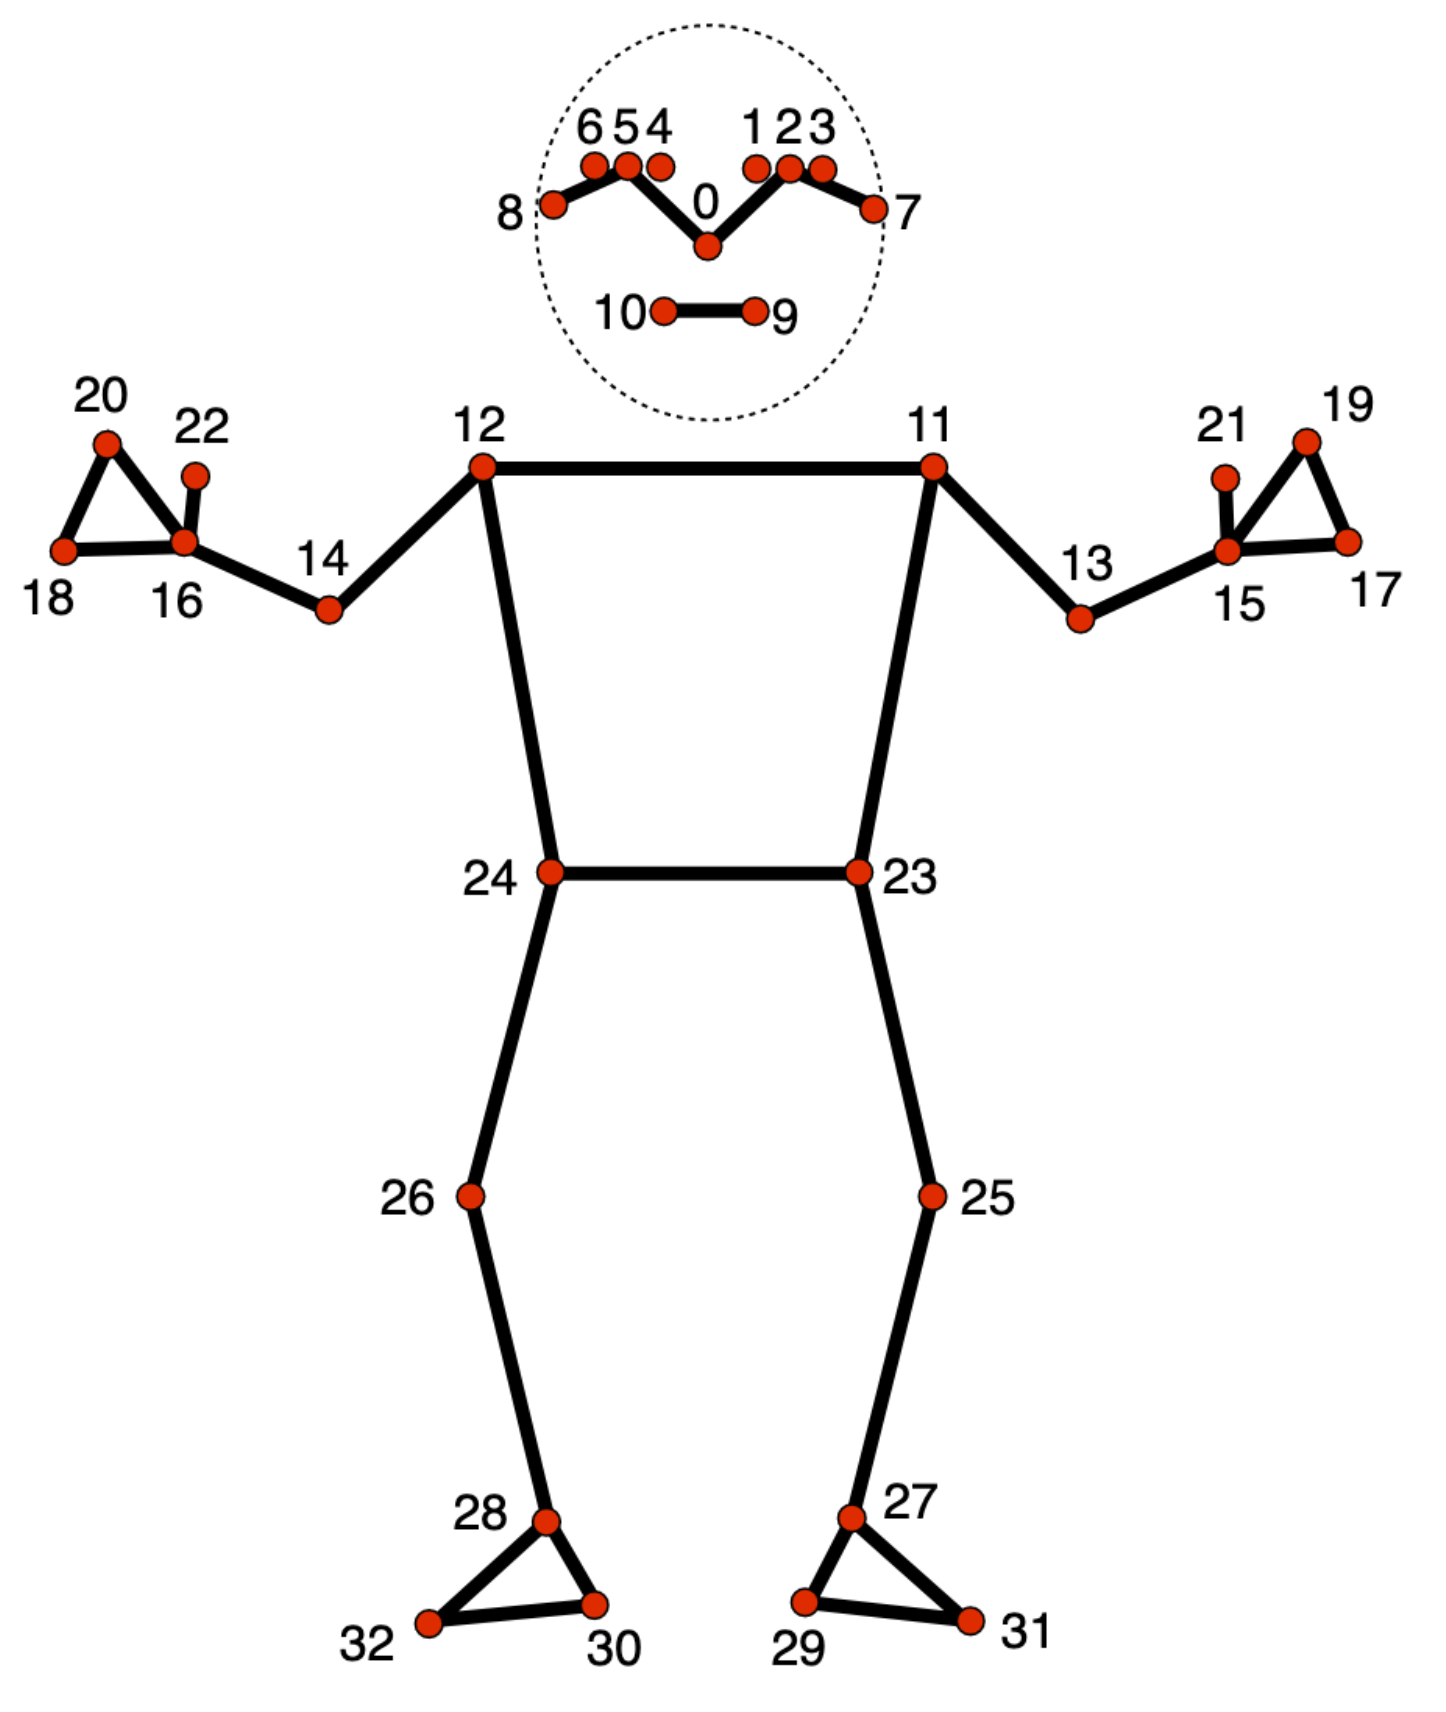
\includegraphics[width=0.9\linewidth]{images/pose_landmarks_index.png}
		% \caption{Landmarks for pose estimation model by MediaPipe}
		\label{fig:pose_landmarks}
	\end{minipage}% <-- Add this percentage sign here
	\begin{minipage}{0.48\textwidth}
		\centering
		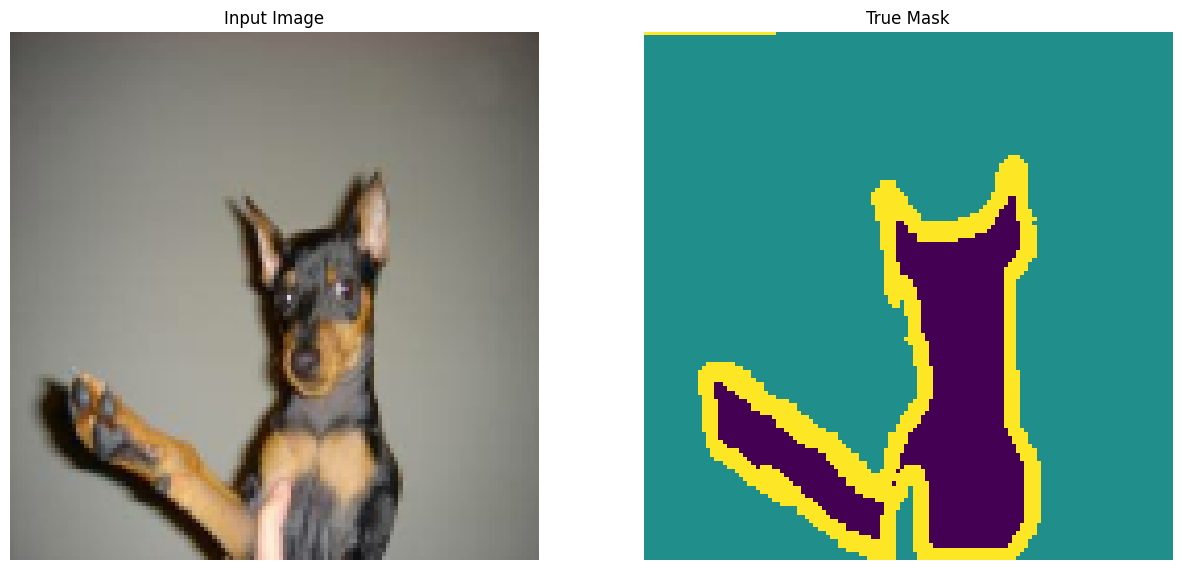
\includegraphics[width=\linewidth]{images/dog.png}
		% \caption{U-Net segmentation on an image from Oxford-IIIT Pet Dataset (Parkhi et al, 2012).}
		\label{fig:dog}
	\end{minipage}
	\caption{Landmarks for pose estimation model by MediaPipe and U-Net segmentation on an image from Oxford-IIIT Pet Dataset (Parkhi et al, 2012).}
	\label{fig:both_figures} % This label can now be used to reference both images together
\end{figure}

\section{Neural Networks}
An artificial intelligence technique called a neural network trains computers to process information like that of the human brain. It uses connected nodes or neurons arranged in a layered pattern to mimic the organization of the human brain. Computers can utilize this adaptive approach to learn from their errors and keep getting better. As a result, artificial neural networks try to more accurately answer challenging problems, such as document summarization and face recognition.
\newline Neural networks consist of neurons in the input layer connected to neurons in the output layer of the network. In Figure \ref{fig:neural_network}, where a general neural network schemes, we can see that they're joined via intermediate neurons. They're placed in hidden layers. 'Hidden' because, in the use of neural networks, only the input and output are of concern to the user. 



\begin{figure}[htp]
	\centering
	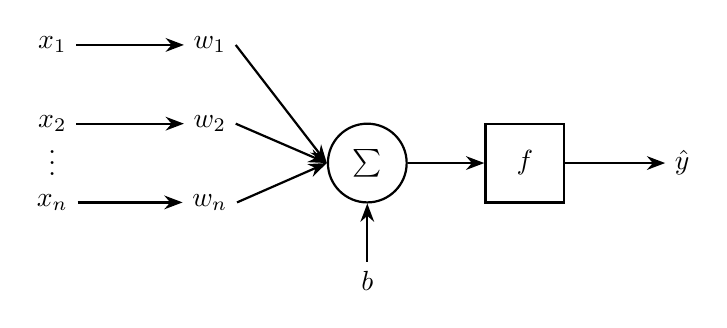
\begin{tikzpicture}[
		>=Stealth,
		input/.style={},
		weights/.style={},
		neuron/.style={
			circle,
			draw,
			thick,
			minimum size=1cm,
			fill=white
		},
		function/.style={
			rectangle,
			draw,
			thick,
			minimum size=1cm
		}
		]
		
		% Inputs
		\node[input] (Input-1) at (0,-1) {$x_1$};
		\node[input] (Input-2) at (0,-2) {$x_2$};
		\node[input] (Input-n) at (0,-3) {$x_n$};
		\node at (0,-2.4) {$\vdots$};
		
		% Weights
		\node[weights] (Weights-1) at (2,-1) {$w_1$};
		\node[weights] (Weights-2) at (2,-2) {$w_2$};
		\node[weights] (Weights-n) at (2,-3) {$w_n$};
		
		% Arrows for weights
		\draw[->, thick] (Input-1) -- (Weights-1);
		\draw[->, thick] (Input-2) -- (Weights-2);
		\draw[->, thick] (Input-n) -- (Weights-n);
		
		% Summation circle
		\node[neuron] (Sum) at (4, -2.5) {$\sum$};
		
		% Bias
		\node[input] (Bias) at (4,-4) {$b$};
		
		% Activation function
		\node[function] (Activation) at (6, -2.5) {$f$};
		
		% Output
		\node[input] (Output) at (8, -2.5) {$\hat{y}$};
		
		% Arrows from weights and bias to sum
		\foreach \i in {1,2,n} {
			\draw[->, thick] (Weights-\i.east) -- (Sum.west);
		}
		\draw[->, thick] (Bias) -- (Sum);
		
		% Arrow from the sum to activation function
		\draw[->, thick] (Sum) -- (Activation);
		
		% Arrow from activation function to output
		\draw[->, thick] (Activation) -- (Output);
		
	\end{tikzpicture}
	
	\caption{Schematic representation of a neuron with inputs, weights, a bias, an activation function, and an output.}
	\label{fig:neuron}
\end{figure}


Neurons are basic building components of neural networks. Each neuron takes inputs ($x_1, x_2, ..., x_n$) which are evaluated by weights ($w_1, w_2, ..., w_n$), which are factors that are changed during training. The weight of the connection affects how much input is passed between neurons. We use the weighted sum of all the inputs, adjusted for the weights of the connections between the inputs and the neuron, to determine the output $\hat{y}$ of the neuron. After summing all inputs multiplied by their weight, a bias $b$ is added. Bias is a constant that shifts the activation function left or right (on x-axis). It tells us how high the weighted sum needs to be before the neuron starts getting meaningfully active. A value that goes into the activation function is then the summation function $\epsilon$,
\begin{equation}
	\epsilon = \sum_{i=1}^{n} x_i w_i + b
	\label{eq:weighted_sum}
\end{equation}
where $n$ is is number of inputs.

\subsection*{Activation Functions}
A neural network's activation function is an essential component. A neural network that lacks an activation function is just a straightforward linear regression model. This indicates that the neural network's non-linearity is provided by the activation function. When computing a weighted some like in \ref{eq:weighted_sum}, we can come out with any number. But for most networks, we want its activations (outputs) to be a value between 0 and 1.\newline
There are many types of activation functions, eg. threshold, sigmoid, rectifier, hyperbolic tangent, and softmax. We'll discuss a few of them.

\subsubsection*{Sigmoid Function}
The data science community is familiar with the sigmoid function from its application in logistic regression. Any value can be entered into the sigmoid function, but it will always return a value between 0 and 1. In image classification tasks, the sigmoid function can be used to convert the linear model's output to probability. This probability can be used to predict the binary classification problem (whether there's a cat or a dog in the image). The sigmoid function has the following mathematical definition:

\begin{equation}
	\sigma(z) = \frac{1} {1 + e^{-z}}
\end{equation}

\subsubsection*{SoftMax Function
}
Softmax function is very similar to a sigmoid function. In multiclass classification problems the sigmoid function isn't useful Applying a threshold for positive prediction of 0.5, would say the input data belongs to two classes. The sigmoid function also doesn't take into account the probability of belonging to other classes, when calculating probability for another class. 

Softmax converts numbers or logits (outputs of neural networks) into probabilities. It works with relative probabilities.

Just like with the sigmoid function, in equation \ref{eq:softmax}, an exponential ensures non-linearity; with $z$ values from the neurons of the output layer for $K$ classes. They are then divided by the sum of exponential values to normalize them before being converted to probabilities. The $i$-th entry can be thought of as the predicted probability of the test input belonging to class i.


\begin{equation}
	\sigma(z_i) = \frac{e^{z_{i}}}{\sum_{j=1}^K e^{z_{j}}} \ \ \ \text{for}\ i=1,2,\dots,K
	\label{eq:softmax}
\end{equation}

\begin{figure}[htp]
	\centering
	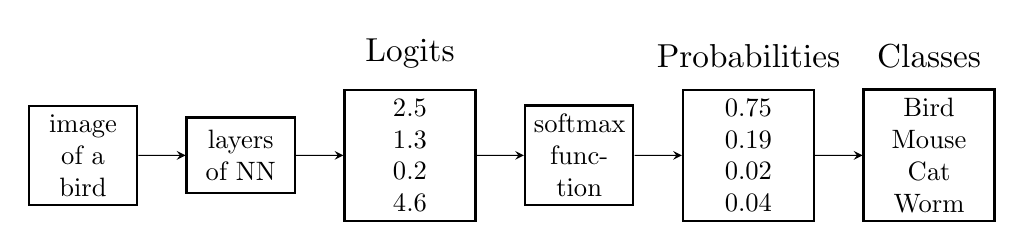
\begin{tikzpicture}[
		box/.style={
			draw,
			thick,
			rectangle,
			minimum height=1cm,
			minimum width=1.2cm, % Reduced width of boxes
			text width=1.2cm,      % Reduced text width inside boxes
			align=center,
			scale=0.8,           % Scale down everything inside the boxes
		},
		node distance=0.5cm,     % Reduced distance between nodes
		scale=1.2,               % Scale the entire tikzpicture
		every node/.style={transform shape} % This ensures that the scaling affects all nodes
		]
		
		% Define nodes
		\node[box] (image) {image of a bird};
		\node[box, right=of image] (layers) {layers of NN};
		\node[box, right=of layers, text width=1.5cm] (logits) {2.5\\1.3\\0.2\\4.6};
		\node[box, right=of logits] (softmax) {softmax function};
		\node[box, right=of softmax, text width=1.5cm] (probabilities) {0.75\\0.19\\0.02\\0.04};
		\node[box, right=of probabilities, text width=1.5cm] (classes) {Bird\\Mouse\\Cat\\Worm};
		
		% Connect nodes
		\draw[-stealth] (image) -- (layers);
		\draw[-stealth] (layers) -- (logits);
		\draw[-stealth] (logits) -- (softmax);
		\draw[-stealth] (softmax) -- (probabilities);
		\draw[-stealth] (probabilities) -- (classes);
		
		% Add titles above boxes
		\node[above=1mm of logits] {Logits};
		\node[above=1mm of probabilities] {Probabilities};
		\node[above=1mm of classes] {Classes};
		
	\end{tikzpicture}
	\caption{A diagram of the NN softmax classification process.}
\end{figure}

\subsubsection*{Rectifier 
	Function}
Unlike the sigmoid function, the rectifier function does not have the same smoothness property. It is still highly used in the deep learning community. The definition of the rectifier function outputs 0 if the input value is less than 0. The function outputs the input if it isn't. It helps to maintain mathematical stability and keep learned values from being stuck around 0 or jumping into infinity.


\begin{equation}
	Relu(x) = max(0, x)
\end{equation}

Rectified Linear Unit activation function, or ReLU for short, is a common term for rectifier function.\newline
While the softmax function works with the output of the last layer of the neural network, the ReLu function is activated in hidden layers.
\begin{figure}[h]
	\centering
	\begin{minipage}{.5\textwidth}
		\centering
		\begin{tikzpicture}
			\begin{axis}[
				width=\linewidth, % Ensures the plot occupies the full width of the minipage
				height=5cm, % Explicit height
				axis lines=middle,
				xmax=10,
				xmin=-10,
				ymin=-0.05,
				ymax=1.05,
				xlabel={$x$},
				ylabel={$y$}
				]
				\addplot [domain=-9.5:9.5, samples=100,
				thick, blue] {1/(1+exp(-x))};
			\end{axis}
		\end{tikzpicture}
	\end{minipage}%
	\begin{minipage}{.5\textwidth}
		\centering
		\begin{tikzpicture}
			\begin{axis}[
				width=\linewidth, % Ensures the plot occupies the full width of the minipage
				height=5cm, % Explicit height
				axis lines=middle,
				xmax=6,
				xmin=-6,
				ymin=-0.05,
				ymax=5.05,
				xlabel={$x$},
				ylabel={$y$},
				xtick={-6, -3, 0, 3, 6},
				ytick={0, 1, 2, 3, 4, 5}
				]
				\addplot [domain=-5.5:5.5, samples=100, thick, blue] {max(0, x)};
			\end{axis}
		\end{tikzpicture}
		
	\end{minipage}
	\caption{Softmax/Sigmoid function and Rectifier function.}
	\label{fig:foftmaxrelu}
\end{figure}

After applying application function $f$, the output of the neuron would then be: 

\begin{equation}
	\hat{y} = f (\epsilon) = f (\sum_{i=1}^{n} x_i w_i + b)
	\label{eq:forpass}
\end{equation}

If we're discussing a neuron in the hidden or output layers, the equation can be rewritten as:

\begin{equation}
	a_i^k =f\left(\sum_{i=1}^{n} w_{ij}^k a_j^{k-1} + b_i^k\right)
	\label{eq:forpasshidden}
\end{equation}

This output is often called an activation $a$. It represents the sum of all neurons in the ($k-1$) layer. The weight $w^k$ is defined for each layer, $k$. The entries of the weights $w^k$ are just the weights connecting to the $k$-th layer of neurons, that is, the entry in the $i$-th row and $j$-th column is $w^k_{ij}$.


\section{Learning}

During training, a function is passed from one neuron to another, either through a function \ref{eq:forpass} for hidden and output layers or through a weighted sum function \ref{eq:weighted_sum} for the input layer. This is known as the forward pass. When the end of the network is reached, the feed-forward is also completed.\newline
The used dataset is commonly split into a training set, on which the model trains, and a validation set, that evaluates the output of the model. 
As the true results are known during the training phase, the error can be calculated by comparing the actual and predicted values. Cost functions are used to obtain an error value.\newline
%cost functions
There are many loss functions used, based on the nature of the problem. A few of them are: mean squared error, used for regression tasks, binary cross entropy, and categorical cross entropy.
\subsubsection*{Cost functions}
As we train the model, we’ll want to evaluate its accuracy using a cost (or loss) function. The cost function tells us about how well our algorithm models our dataset. The loss error is calculated for each training sample, while the loss function represents the whole set of $m$ samples. The cost function represents the average loss error for a sample. It is a function that assesses how well an ML model performs with a given set of data. The error between expected and predicted values is quantified by the cost function and shown as a single real number. Cost functions can be formed in a variety of ways, depending on the nature of the problem.
\paragraph{Mean squared error}\mbox{}\\
For a model using a formula \ref{eq:forpasshidden},
the commonly used loss function used for regression tasks, is the mean squared error (MSE). 
The cost for a single training example x may be written as


\begin{equation}
	MSE = \frac{1}{2m} \sum_{i=1}^{m} (y_i - a_i)^2,
\end{equation}
where
$i$ represents the index of the sample,
$a$ is the predicted outcome,
$y$ is the actual value, and
$m$ is the number of samples.

\paragraph{Crossentropy function}\mbox{}\\
Other names for cross-entropy loss include logistic loss, log loss, and logarithmic loss. Every predicted class probability is compared to the actual class probability, and a loss function is used to penalize the probability according to its deviation from the actual expected value. Because the penalty is logarithmic, large differences near 1 will result in a large score, and small differences approaching 0 will result in a small score. Cross-entropy loss in a perfect model is 0.
What is meant by cross-entropy is:
\begin{equation}
	-\sum_{c=1}^My_{o,c}\log(p_{o,c}),
\end{equation}
where $M$ is number of classes, $y$ is the binary indicator if class of label $c$ is the correct classification for observation $o$ and $p$ is the predicted probability.

When dealing with labels that are one-hot encoded, such as the 3-class classification problem, where the values are [1,0,0], [0,1,0], and [0,0,1], categorical cross-entropy is employed.
Labels in sparse categorical cross-entropy are encoded with integers, such as [1], [2], and [3] for a 3-class problem.



There are many other types of cost functions used in ML, e.g. Root Mean Square error (RMSE), Binary Cross Entropy Loss Function,  Categorical cross-entropy, Hinge Loss, Kullback-Liebler Divergence LOSS (KL-Divergence), and Huber Loss. Choosing a cost function will be influenced by the type of problem, the output activation function, and the network architecture.


%koniec cost functions
With multi-class, single-label classification problems, as we'll deal with, the first choices of activation and loss functions are ReLU for hidden layers, softmax for the last layer, and categorical crossentropy as a loss function.



The training of a neural network begins with the random assignment of weights and biases (usually to 0) between the nodes. After the initial forward pass, the output layer is highly variable and lacks an identifiable pattern. To address this, a cost function is used to determine the error between the output and the desired values. 

The goal is to enable the computer to find appropriate settings for all of the parameters - weights and biases. That also means minimizing the cost function. \newline
In ML, minimizing the cost (loss) function is done by optimizers. Common optimizers include gradient descent, stochastic gradient descent, or Adam optimizer.


\textbf{Gradient Descent} is a fundamental optimization algorithm used in classification problems and linear regression. It calculates the first derivatives of the cost function to find the minimum. 
Each negative gradient component provides two pieces of information. The sign indicates whether the corresponding input vector component should be increased or decreased. Importantly, the relative magnitudes of all the components indicate which changes are more significant for the cost function output.
However, Gradient Descent may sometimes be trapped in a local minimum and unable to determine the global minimum.\\
\textbf{Stochastic gradient} descent algorithms are a variant of the gradient descent method used in ML. In stochastic gradient descent, instead of computing the gradient using all the observations, only a small random sample of the training data is used to estimate the gradient. This method can significantly reduce the computation time, making it a useful approach in many machine learning applications.\\
\textbf{Adam} is convenient for most convex optimization problems with large datasets. It combines adaptive methods and momentum methods, where it takes into account the moving average of the gradient's first and second-order moments. This allows it to effectively adapt the learning rates for each parameter.
It is an extension of stochastic gradient descent.\newline
Minimizing the cost functions means a better performance on all samples. The algorithm for computing the gradient efficiently is called the backpropagation.
\subsubsection*{Backpropagation}
The backpropagation algorithm is the foundation of neural network learning. The goal of backpropagation is to understand how altering the weights and biases in a network alters the cost function. \newline
In backpropagation, the partial derivatives $\partial C / \partial w^k_{ij}$ and $\partial C / \partial b^k_i$ are computed, calling $C$ the cost. \newline
Let's say we work with a cost function (MSE) for one training example in a simple network, such as in Figure \ref{fig:backprop}: $C_0 (w_1, w_2, \dots, w_{n}) = (a^k - y)^2$.\newline
\begin{figure}
	\centering
	\begin{tikzpicture}[node distance=1.5cm, auto]
		% Define nodes
		\node (a) {\( a^{(k-1)} \)};
		\node[below of=a] (w) {\( w^{(k)} \)};
		\node[right of=w] (z) {\( \epsilon^k \)};
		\node[right of=z] (aL) {\( a^{(k)} \)};
		\node[below of=w] (b) {\( b^k\)};
		\node[right of=aL] (C) {\( \color{red} C_0 \)};
		\node[below of=C] (y) {\( y \)};
		
		% Draw arrows
		\draw[->] (a) -- (z);
		\draw[->] (w) -- (z);
		\draw[->] (z) -- (aL);
		\draw[->] (aL) -- (C);
		\draw[->] (b) -- (z);
		\draw[->] (y) -- (C);
	\end{tikzpicture}
	\caption{An example structure for backpropagation.}
	\label{fig:backprop}
\end{figure}
We want to find the effect of the weight change on the cost function. In ML, the chain rule is often considered in the context of networks.
The last activation $a^k$ is determined by the weighted sum $\epsilon^k$, or a weight $w^k$ multiplied by the previous neuron's activation $a^{(k-1)}$ plus some bias $b^k$. After an activation function, $a^k = f(\epsilon^k)$. These parameters, along with a constant $y$ (wanted output), let us compute the cost.\newline
If the question is how sensitive the cost function is to small changes in our weight $w^k$, we simply calculate the derivative of $C_0$ with respect to $w^k$, using the chain rule.
The equation is as follows:
\begin{equation} 
	\frac{\partial C_0 }{\partial w^k} = 
	{\color{magenta}\frac{\partial \epsilon^k }{\partial w^k}} 
	{\color{violet}\frac{\partial a^k }{\partial \epsilon^k}} 
	{\color{blue}\frac{\partial C_0 }{\partial a^k}} 
\end{equation}
With the computed derivatives:
\begin{equation}
	\frac{\partial C_0}{\partial w^k} =
	{\color{magenta}a^{(k-1)}}
	{\color{violet}f'(\epsilon^k)}
	{\color{blue}2(a^k - y)}
\end{equation}
It's worth noting that the last derivative multiplies the difference between the network's output and the thing we want it to be, so if that output is very different, even slight changes stand to have a big impact on the final cost.\newline
This was computed only for a single training example. Since the full cost function involves averaging together all the cost across many different training examples, its derivative requires averaging the expression over all $n$ training examples:
\begin{equation*}
	\frac{\partial C}{\partial w^{k}} = \frac{1}{n} \sum_{i=0}^{n-1} \frac{\partial C_i}{\partial w^{k}}
\end{equation*}
Of course, that is just one component $w^k$ (in layer $k$) of the gradient vector $\nabla C$, which itself is built up from partial derivatives of the cost function with respect to all the weights and biases.
The sensitivity to bias is almost identical:
\begin{equation*}
	\frac{\partial C_0}{\partial b^{k}} = \frac{\partial \epsilon^{k}}{\partial b^{k}} \frac{\partial a^{k}}{\partial \epsilon^{k}} \frac{\partial C_0}{\partial a^{k}} = 1 \cdot f'(\epsilon^{k}) \cdot 2(a^{k} - y)
\end{equation*}
We want to see how sensitive this cost function is to the activation of the previous layer. The derivative of the weighted sum $\epsilon$ with respect to the activation in the previous layer, comes out to be the the weight.

\begin{equation*}
	\frac{\partial C_0}{\partial a^{(k-1)}} = \frac{\partial \epsilon^{k}}{\partial a^{(k-1)}} \frac{\partial a^{k}}{\partial z^{k}} \frac{\partial C_0}{\partial a^{k}} = w^{k} f'(\epsilon^{k}) 2(a^{k} - y)
\end{equation*}


When $\partial C / \partial \epsilon_i^k$ is close to 0, we can say that the neuron is already near optimal.
Let's call $C$ a cost function for an average weight or a bias, and $-\nabla C$ a negative gradient of the cost function. 
\begin{equation}
	-\nabla C(w_1, w_2, \dots, w_{n}) = 
	\begin{bmatrix}
		-0.08 \\
		+0.12 \\
		-1.06 \\
		\vdots \\
		+0.04
	\end{bmatrix}
	\label{eq:nabla}
\end{equation}

In equation \ref{eq:nabla}, the negative gradients for each weight (their average), are already calculated. So for the cost function to get closer to a minimum, the weights need to be changed accordingly. The cost function is sensitive to the weight $w_1$ of $0.08$. 
After this is computed the weight just needs to be updated in the way:
\begin{equation*}
	w_1= w_1 -\alpha \frac{\partial C}{\partial w_1} ,
\end{equation*}

Where $\alpha$ is a learning rate, which determines the gradient’s influence, and $\frac{\partial C}{\partial w_1} $ is the partial derivative of the cost function $C$ with respect to $w_1$.\newline
In summary, the training can be divided into a few steps:
\begin{enumerate}[label=\arabic*.]
	\item Forward Pass til the final predictions are made.
	\item Loss Calculation
	\item Backward Pass (Backpropagation)
	\item Weight Update
\end{enumerate}
This entire process is repeated for a specified number of epochs or until another stopping criterion is met (like the early stopping callback, which halts training if the validation loss doesn't improve for a set number of epochs).
\begin{figure}[htp]
	\centering
	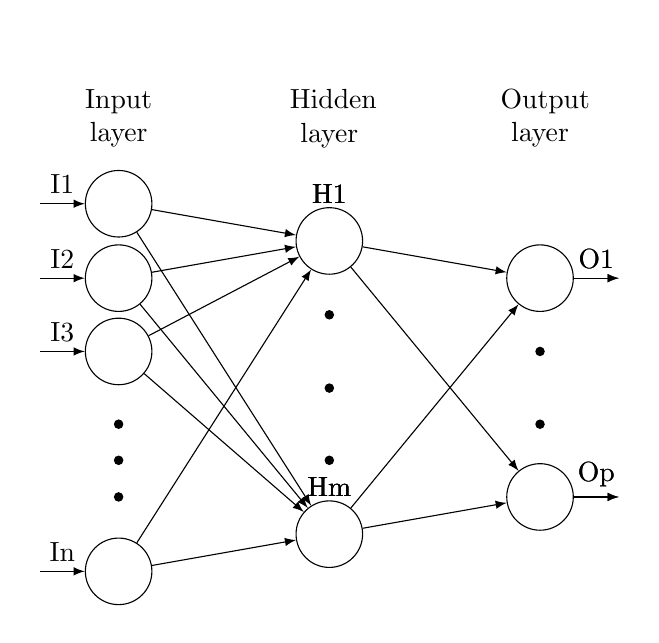
\begin{tikzpicture}[
		plain/.style={
			draw=none,
			fill=none,
		},
		dot/.style={draw,shape=circle,minimum size=3pt,inner sep=0,fill=black
		},
		net/.style={
			matrix of nodes,
			nodes={
				draw,
				circle,
				inner sep=8.5pt
			},
			nodes in empty cells,
			column sep=0.6cm,
			row sep=-11pt
		},
		>=latex
		]
		\matrix[net] (mat)
		{
			|[plain]| \parbox{1cm}{\centering Input\\layer}
			& |[plain]| \parbox{1cm}{\centering Hidden\\layer}
			& |[plain]| \parbox{1cm}{\centering Output\\layer} \\
			& |[plain]|                 \\
			|[plain]| &            & |[plain]|    \\
			& |[plain]|  &              \\
			|[plain]| & |[dot]|                   \\
			& |[plain]|  & |[dot]|      \\
			|[plain]| & |[dot]|    & |[plain]|    \\
			|[dot]|   & |[plain]|  & |[dot]|      \\
			|[dot]|   & |[dot]|    & |[plain]|    \\
			|[dot]|   & |[plain]|  &              \\
			|[plain]| &            & |[plain]|    \\
			& |[plain]|                 \\
		};
		\foreach \ai/\mi in {2/I1,4/I2,6/I3,12/In}
		\draw[<-] (mat-\ai-1) -- node[above] {\mi} +(-1cm,0);
		\foreach \ai in {2,4,6,12}
		{\foreach \aii/\mii in {3/H1,11/Hm}
			\draw[->] (mat-\ai-1) -- (mat-\aii-2) node[yshift=0.6cm] {\mii};
		}
		\foreach \ai in {3,11}
		{  \draw[->] (mat-\ai-2) -- (mat-4-3);
			\draw[->] (mat-4-3) -- node[above] {O1} +(1cm,0);}
		\foreach \ai in {3,11}
		{  \draw[->] (mat-\ai-2) -- (mat-10-3);
			\draw[->] (mat-10-3) -- node[above] {Op} +(1cm,0);}
	\end{tikzpicture}
	
	\caption{Structure of neural network}
	\label{neural_n_example}
\end{figure}
\subsection*{Hyperparameters of Neural Networks}
\begin{itemize}
	\item Learning Rate is a crucial parameter that controls to which extent the model needs to be modified. It determines the step size at each training iteration. It is usually a value between 0 and 1. We can determine the direction of a loss function's optimum by computing the loss function's gradient. The step size in that direction is determined by the learning rate parameter.
	\item Batch size tells us how much data is changed during 1 cycle (one epoch) of training. The data is subdivided into batches and each step is computed with respect to a batch. Larger batch sizes could lead to faster training but with a trade-off for lower accuracy or overfitting. The best size will depend on several variables, such as the size of the training dataset, the complexity of the model, and the available computational resources.
	\item Epochs define the number of times that the learning algorithm will work through the entire training dataset. Every sample in the training dataset has had a chance to update the internal model parameters after one epoch. One or more batches make up an epoch.
\end{itemize}
\subsubsection*{Regulations of Neural Network}
When talking about the regulation of neural networks we can mention techniques like dropout or early stopping.\newline
Dropout is a regularization strategy for neural networks that, with a given probability, drops a unit (along with connections) during training. It randomly sets a fraction of inputs to 0 at each update during training.
The goal is to stop co-adaptation, which occurs when a neural network becomes overly dependent on a single connection and may be an indication of overfitting. It makes intuitive sense to think of dropout as the formation of an implicit neural network ensemble. The result of dropout is shown in Figure \ref{fig:dropout}
\def\layersep{2}
\def\nodesep{1.5}
\begin{figure}[htp]
	\centering
	\begin{tikzpicture}[
		node/.style={circle, draw, thick},
		scale=0.7, % Adjust the scaling factor as needed
		transform shape,
		every node/.style={scale=0.8} % Adjust the node text scaling factor as needed
		]
		
		\foreach \y in {1,...,5}{
			\node[node] (i\y) at (0,\nodesep*\y) {};
			\node[node, right=\layersep of i\y] (h1\y) {};
			\node[node, right=\layersep of h1\y] (h2\y) {};
		}
		
		\node[node, right=\layersep of h22] (o1) {};
		\node[node, right=\layersep of h24] (o2) {};
		
		\foreach \source in {1,...,5}
		\foreach \dest in {1,...,5}{
			\path[-stealth, thick] (i\source) edge (h1\dest);
			\path[-stealth, thick] (h1\source) edge (h2\dest);
		}
		\foreach \source in {1,...,5}
		\foreach \dest in {1,2}
		\draw[-stealth, thick] (h2\source) -- (o\dest);
		
		\draw[-stealth, thick] (7.5,3*\nodesep) -- node[above,font=\Large] {dropout} (9.5, 3*\nodesep);
		
		% Boundary
		
		\foreach \y in {1,...,5}
		\node[node, right=15em of h2\y] (di\y) {};
		
		\node[red,font=\huge] at (di1) {$\times$};
		\node[red,font=\huge] at (di3) {$\times$};
		
		\foreach \y in {1,...,5}
		\node[node, right=\layersep of di\y] (dh1\y) {};
		
		\node[red,font=\huge] at (dh11) {$\times$};
		\node[red,font=\huge] at (dh13) {$\times$};
		\node[red,font=\huge] at (dh14) {$\times$};
		
		\foreach \y in {1,...,5}
		\node[node, right=\layersep of dh1\y] (dh2\y) {};
		
		\node[red,font=\huge] at (dh22) {$\times$};
		\node[red,font=\huge] at (dh24) {$\times$};
		
		\node[node, right=\layersep of dh22] (do1) {};
		\node[node, right=\layersep of dh24] (do2) {};
		
		\foreach \source in {2,4,5}
		\foreach \dest in {2,5}
		\draw[-stealth, thick] (di\source) -- (dh1\dest);
		
		\foreach \source in {2,5}
		\foreach \dest in {1,3,5}
		\draw[-stealth, thick] (dh1\source) -- (dh2\dest);
		
		\foreach \source in {1,3,5}
		\foreach \dest in {1,2}
		\draw[-stealth, thick] (dh2\source) -- (do\dest);
		
	\end{tikzpicture}
	\caption{Visualization of dropout.}
	\label{fig:dropout}
\end{figure}
\newline An intuitive technique for training just enough is early stopping. It prevents the model from learning on a 'noised' dataset. When training, after every epoch, the model is evaluated using a validation dataset. The training process is terminated if the model's performance on the validation dataset begins to drop (for example, if loss starts to rise or accuracy starts to fall).





%types of models
%neural networks

%use and so on, how works
%rgb gbr conversion

%\section{Types of classifiers and models for Computer Vision}
%An algorithm, or the set of rules that robots employ to classify data, is called a classifier. %However, the final result of the classifier's machine learning is a classification model. The %data is first classified by the model, which was trained using the classifier.






%\subsection{Input Image Processing}
%color, background, extracting landmarks for mediapipe model no. 2, with vs without Mediapipe




\iffalse
/*\section{Gesture Recognition}

Gesture recognition is the practice of identifying hand gestures as input, and translating them into a meaningful command for devices. Dynamic gestures involve a series of changing poses, whereas static gestures remain fixed. Our focus is on recognizing static gestures via a vision-based approach. Vision-based gesture recognition technology is a growing field of study, researchers have developed various methods for feature extraction, including geometric features, moment features, contour features, histograms of oriented gradients, and wavelet features. Examples include a geometric descriptor based on lines connecting the hand contour\cite{lopez2019gesture}, a method based on hand shape \cite{article}, masked Zernike moment features \cite{park2014hand}, geometry-based normalizations \cite{priyal2013robust}, edge orientation histograms. Other techniques include saliency-based features, sparse representation, and geometric features. The recognition algorithm used in these studies includes a weighted AdaBoost classifier based on finger-earth mover's distance and SVM models. Deep learning-based neural networks have shown potential in recognizing hand gestures, using methods like segmented binary images, restricted Boltzmann Machines, pose-guided ensemble networks, and hybrid feature attention networks. However, these methods are not robust enough to handle the complexity of hand gesture images in unconstrained environments.


\fi





%practice
\chapter{Practical Part}
In this chapter, we discuss the implementation of a gesture recognition system utilizing the MediaPipe framework. We look into our neural network model and its results with a comprehensive analysis of the model's performance. Furthermore, the chapter includes a comparison of various machine learning optimizers, highlighting their impact on the training dynamics and outcomes of the model. We also discuss how the gesture recognition model is applied in real-world scenarios, controlling a Tello drone through recognized gestures. This practical application demonstrates how gestures can directly influence drone behavior for tasks such as navigation and interaction, bridging the gap between theoretical development and real-world application.
\section{Mediapipe}
MediaPipe is a framework used to create machine learning pipelines for time-series data like video and audio. Google initially developed it to process real-time video and audio analysis on YouTube \cite{mediapipe2019blog}. In 2019, the public release allowed researchers and developers to incorporate MediaPipe into their projects. Unlike other machine learning frameworks that require high computing power, MediaPipe can run efficiently on devices with low power, such as Android and IoT devices. It consists of the MediaPipe framework and MediaPipe solutions. The MediaPipe framework is developed using C++, Java, and Objective C programming. MediaPipe solutions include 16 pre-trained TensorFlow and TensorFlow Lite models built on top of the MediaPipe framework for specific use cases.
\subsection{MediaPipe Hands}
MediaPipe Hands is a solution that tracks hands in real-time. The problem of detecting hands is somewhat intricate. The model must be able to recognize hands and it must function across a wide range of hand sizes with a big scale span so it must be robust. It is rather difficult to identify hands based just on their visual traits since hands lack high-contrast patterns.% found on faces, such as those surrounding the lips and eyes.

MediaPipe Hands utilizes a combination of object detection, classification, and regression to recognize and track hands within a given image or video frame. The pipeline consists of two convolutional neural network models: a palm detector and a hand landmark model.


The palm detector is a single-shot detector model that uses an orientated hand-bounding box to locate palms on a whole input image. This is done before landmark detection because it is easier to estimate bounding boxes of rigid objects like palms than detecting hands with articulated fingers. It ignores many aspect ratios and so the bounding boxes are only squared. The model uses both classification (hands, no hands), and object detection (predicting a bounding box around the detected hand), a focal loss \cite{DBLP:journals/corr/abs-1708-02002} It was trained on data, containing 700 images of 14 geographical subregions, from both men and women.


The Hand Landmark Model runs subsequently with the palm detection model and uses regression to precisely localize 21 3D (x, y, z) coordinates within the hand region, similar to the data glove \ref{txt:glove}. Each landmark has a specific location on the hand that can vary within the pixel grid of an image. To capture the exact position, continuous values are used, allowing the model to indicate precisely where each landmark is located on the hand in terms of its x and y (and possibly z) coordinates within the image. The hands move and rotate freely, leading to a wide range of possible positions and orientations for each landmark. Continuous values are used because they make it possible to track hand gestures and movements more precisely. These gestures and movements may involve tiny changes to position and orientation that would be lost in discretized values.
The model is resilient to self-occlusions and partially visible hands, and it learns a consistent internal hand posture representation. The results from the model contain 21 hand landmarks consisting of x, y, and z, a hand flag that indicates the likelihood that a hand is present in the input image, and a binary system of handedness, e.g. left or right hand.
The coordinates x and y for each landmark are normalized \ref{sec:norm} to [0, 1] by image width and height. 

The model was trained both on real-world and synthetic datasets, noting that the wrist point was learned only from synthetic images. More than 30,000 manually annotated real-world images were used and the model is very robust, allowing it to detect and map hand landmark points accurately, even on partially visible hands in most cases. In Figure
\ref{fig:landmark_both_hands} my hands are not facing upfront but the model still finds all the landmarks for both hands. If tracking 2 hands, it also shows which one is left or right with different colors.

For encountering a tracking failure, There was also another model output created for tracking failures. It generates the likelihood that the given crop contains a hand that is reasonably aligned. The detector is triggered to reset tracking if the score falls below a predetermined threshold.

\begin{figure}
	\centering
	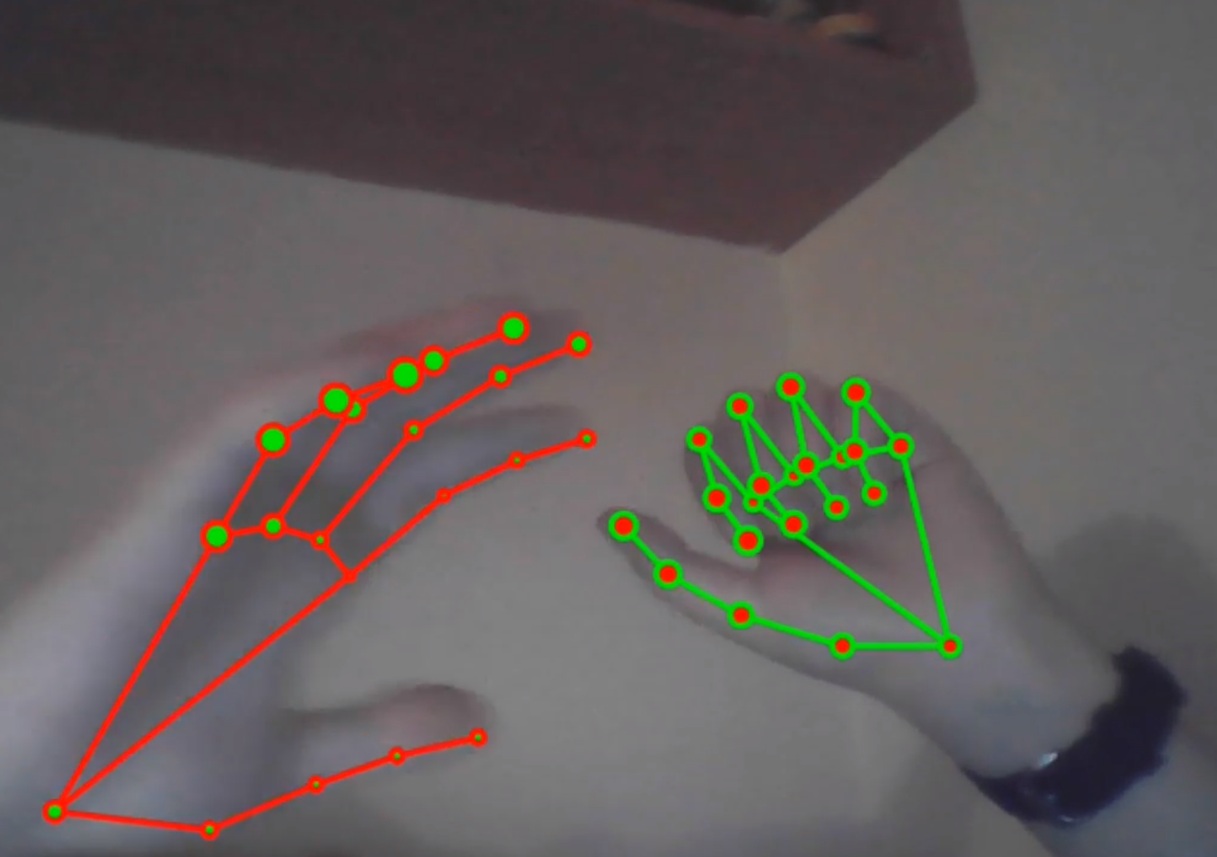
\includegraphics[width = 0.5\textwidth]{images/landmarks_both_hands.png}
	\caption{Hand landmarks model output}
	\label{fig:landmark_both_hands}
\end{figure}

% Ensure the subsection does not end with the figure
\par~
\newline

\subsubsection*{Data Normalization}\label{sec:norm}
The MediaPipe hand landmarks model provides coordinates for hand landmark points based on the position of pixels containing those points in an image. As a result, the coordinates of two images of the same hand sign with different placements in the frame can have significantly different distances between them. This makes it more challenging to train the model.

To solve this problem, the wrist's landmark point has been considered with coordinates [0,0], and the coordinates of all other landmark points were adjusted accordingly.
First, the coordinates' values of the wrist's landmark point are subtracted from all coordinates' values.

Then, the coordinates were normalized to be between 0 and 1 by dividing them by the largest absolute value of the difference. Finally, the normalized coordinates were collected in the landmarks list. The coordinate normalization procedure is shown in Figure \ref{fig:normalization}.


\begin{figure}
	\centering
	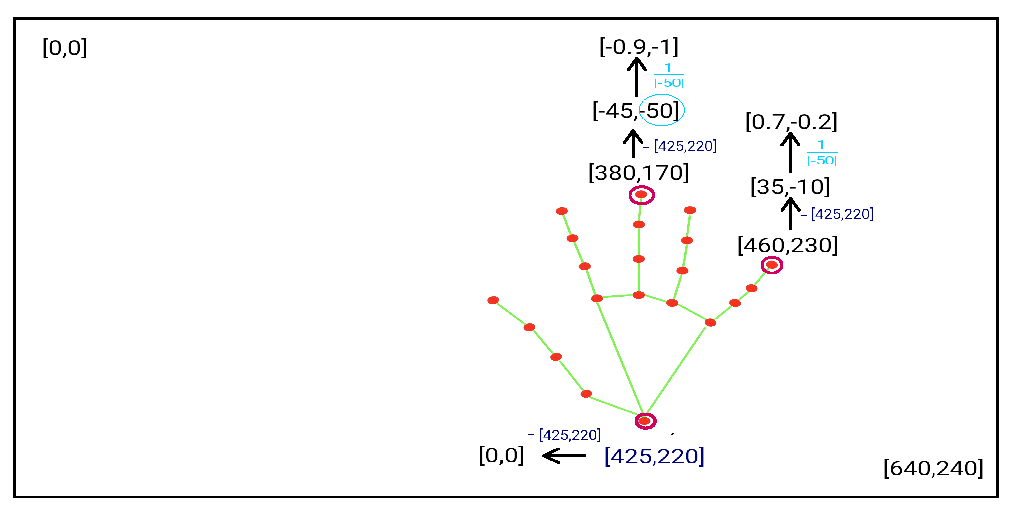
\includegraphics[width = 0.85\textwidth]{images/normalise.pdf}
	\caption{Process of normalization of landmark coordinates}
	\label{fig:normalization}
\end{figure}

\subsection{MediaPipe Face}
With support for multiple faces and six landmarks (left eye, right eye, nose tip, mouth, left eye region, and right eye region), MediaPipe Face Detection is a quick solution for face detection. Mediapipe BlazeFace \cite{bazarevsky2019blazeface} is a compact and efficient face detector designed for mobile GPU inference, that serves as its foundation, detecting only a few landmarks on the face and drawing a bounding box. Because of its real-time performance, the detector can be used with any live viewfinder experience that needs a precise facial region of interest as an input for other task-specific models, like face region segmentation, facial feature or expression classification, and 3D facial geometry estimation (like MediaPipe Face Mesh). BlazeFace leverages a resolution technique as an alternative to a GPU-friendly anchor mechanism adapted from Single Shot MultiBox Detector (SSD) \cite{Liu_2016} and a lightweight feature extraction network that is similar to MobileNetV1/V2 \cite{howard2017mobilenets}. With BlazeFace in use, we can get outputs shown in Figure \ref{fig:face_detections}, also outputting the confidence of the face.


\begin{figure}[ht]
	\centering
	\begin{minipage}{0.5\textwidth}
		\centering
		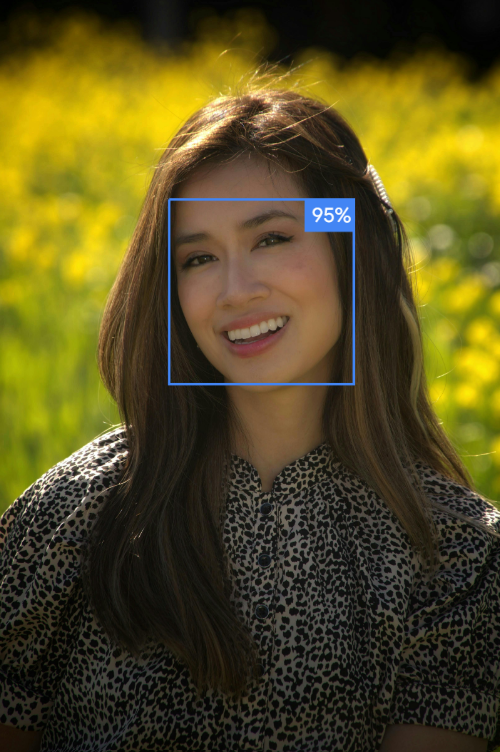
\includegraphics[width=0.5\textwidth]{images/face_detection_good.png}
		%   \caption{Landmarks for pose estimation model by MediaPipe}
	\end{minipage}% <-- This percentage sign denotes the end of a minipage
	\begin{minipage}{0.5\textwidth}
		\centering
		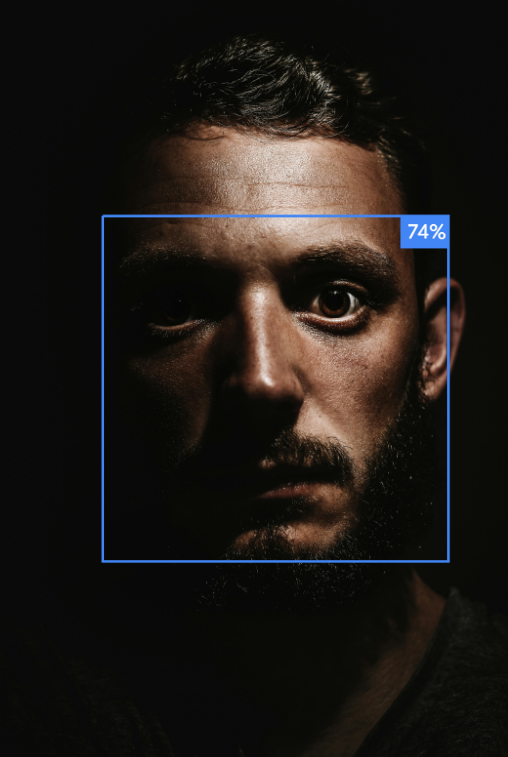
\includegraphics[width=0.5\textwidth]{images/face_detection.png}
		%   \caption{U-Net segmentation on an image from Oxford-IIIT Pet Dataset (Parkhi et al, 2012).}
	\end{minipage}
	\caption{Outputs of face detection model with different lightings}
	\label{fig:face_detections} % This label can now be used to reference both images together
\end{figure}


\section{Data Collection}

To make predictions, we had to train our model with data. Since we decided to use hand gestures, we had to collect the data ourselves. After finishing the training, we established drone commands and tested our program.

Although many publicly accessible datasets contain pictures of hand gestures, we chose to collect our data using the MediaPipe hand-tracking model. To do this, we recorded video footage of various hand gestures being held for a specific duration and moved around to increase diversity. Because the MediaPipe models are open-sourced and many developers use them for various projects, there are also numerous programs available for capturing and labeling gestures, like \cite{opencv_mediapipe_hand_gesture_recognition}.
\begin{figure}[h!]
	\centering
	\includegraphics[width = \textwidth]{images/all_gestures.pdf}
	\caption{Gestures used in this project.}
	\label{fig:all_gestures}
\end{figure}


 During the recording process, we labeled each gesture by pressing a key. Our dataset includes over 5000 samples, including images of both right and left hands, palms facing forward or backward toward the camera, and various degrees of hand positions captured by the camera.



Our final dataset has 8 total classes. It demonstrates the efficacy of the model and minimizes the risk of error commands that could lead to unsafe situations. The gestures are shown in Figure \ref{fig:all_gestures}.


\begin{table}[h]
	\centering
	\caption{A selection of the saved csv file}
	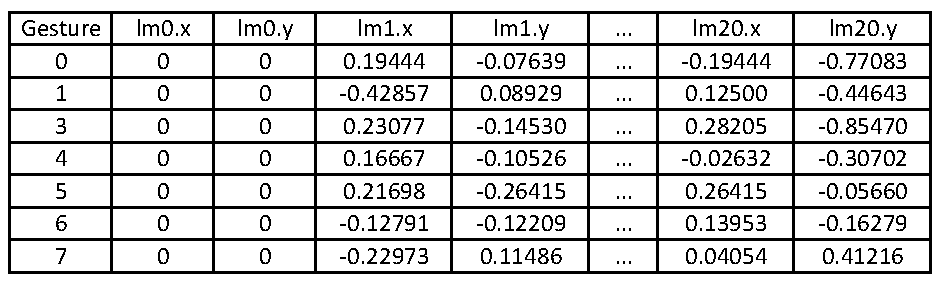
\includegraphics[width = \textwidth]{images/gesture_laandmarks-cropped.pdf}
	\label{tab:saved_csv} % Use tab: prefix for table labels
\end{table}


The hand-tracking model used for data collection, outputs x, y, and z coordinates of hand landmark points from images, but only x and y coordinates are necessary for training the final model. Therefore, we eliminated the z coordinates. After normalization \ref{sec:norm}, we stored the remaining x and y coordinates of hand landmarks for various hand signs in a csv file for each hand landmark. The coordinates displayed in Figure \ref{tab:saved_csv} represent the data points used to generate the final dataset and train the final model. The first column denotes the gesture label, the next two columns indicate the coordinates of landmark 0 at the wrist, and so on. Our csv file contains many combinations of landmark coordinates for each gesture.

 



\section{Model}
\begin{figure}[ht]
	\centering
	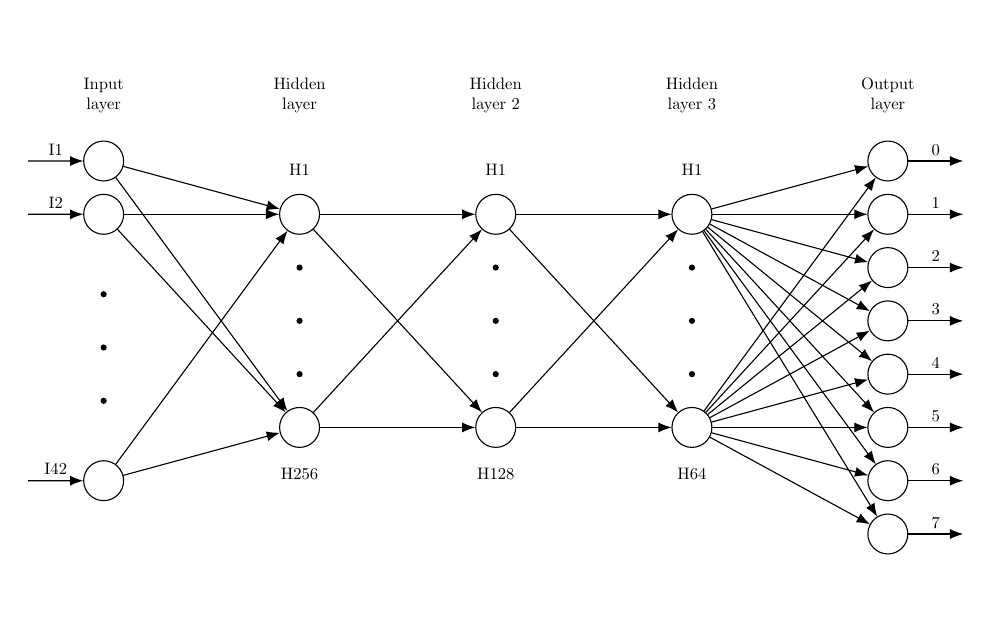
\begin{tikzpicture}[
		scale = 0.7,
		every node/.style={scale=0.6},
		plain/.style={
			draw=none,
			fill=none,
		},
		cir/.style={
			draw,
			circle,
			inner sep=8.5pt
		},
		dot/.style={
			draw,
			shape=circle,
			minimum size=3pt,
			inner sep=0,
			fill=black
		},
		net/.style={
			matrix of nodes,
			nodes={
				draw,
				circle,
				inner sep=8.5pt
			},
			nodes in empty cells,
			column sep=1cm,
			row sep=-5pt
		},
		arrow/.style={-Latex}
		]
		\matrix[net] (mat)%10x5
		{
			|[plain]| \parbox{1.5cm}{\centering Input\\layer}
			& |[plain]| \parbox{1.5cm}{\centering Hidden\\layer}
			& |[plain]| \parbox{1.5cm}{\centering Hidden\\layer 2}
			& |[plain]| \parbox{1.5cm}{\centering Hidden\\layer 3}
			& |[plain]| \parbox{1.5cm}{\centering Output\\layer} \\
			|[cir]| &           |[plain]| &     |[plain]| &         |[plain]| &             |[cir]| \\
			|[plain]| &         |[plain]| &     |[plain]| &         |[plain]| &               |[plain]| \\
			|[cir]| &           |[cir]| &       |[cir]| &         |[cir]| &             |[cir]| \\
			|[plain]| &         |[plain]| &       |[plain]| &           |[plain]| &               |[plain]| \\
			|[plain]| &         |[dot]| &       |[dot]| &           |[dot]| &               |[cir]| \\
			|[dot]| &           |[plain]|   &     |[plain]| &           |[plain]| &               |[plain]| \\
			|[plain]| &         |[dot]| &     |[dot]| &         |[dot]| &             |[cir]| \\
			|[dot]| &           |[plain]| &       |[plain]| &           |[plain]| &               |[plain]| \\
			|[plain]| &         |[dot]| &     |[dot]| &         |[dot]| &             |[cir]| \\
			|[dot]| &           |[plain]| &     |[plain]| &         |[plain]| &             |[plain]| \\
			|[plain]| &         |[cir]| &       |[cir]| &           |[cir]| &               |[cir]| \\
			|[plain]| &         |[plain]| &     |[plain]| &         |[plain]| &             |[plain]| \\
			|[cir]| &           |[plain]| &     |[plain]| &         |[plain]| &             |[cir]| \\
			|[plain]| &         |[plain]| &     |[plain]| &         |[plain]| &             |[plain]| \\
			|[plain]| &         |[plain]| &     |[plain]| &         |[plain]| &             |[cir]| \\
			|[plain]| &         |[plain]| &     |[plain]| &         |[plain]| &             |[plain]| \\
		};
		
		% Connect the 'cir' nodes from Input Layer to Hidden Layer 1
		\draw[arrow] (mat-2-1) -- (mat-4-2);
		\draw[arrow] (mat-2-1) -- (mat-12-2);
		\draw[arrow] (mat-4-1) -- (mat-12-2);
		\draw[arrow] (mat-4-1) -- (mat-4-2);
		\draw[arrow] (mat-14-1) -- (mat-4-2);
		\draw[arrow] (mat-14-1) -- (mat-12-2);
		
		% Connect the 'cir' nodes from Hidden Layer 1 to Hidden Layer 2
		\draw[arrow] (mat-4-2) -- (mat-4-3);
		\draw[arrow] (mat-4-2) -- (mat-12-3);
		\draw[arrow] (mat-12-2) -- (mat-12-3);
		\draw[arrow] (mat-12-2) -- (mat-4-3);
		
		
		% Connect the 'cir' nodes from Hidden Layer 2 to Hidden Layer 3
		\draw[arrow] (mat-4-3) -- (mat-4-4);
		\draw[arrow] (mat-4-3) -- (mat-12-4);
		\draw[arrow] (mat-12-3) -- (mat-12-4);
		\draw[arrow] (mat-12-3) -- (mat-4-4);
		
		% Connect the 'cir' nodes from Hidden Layer 3 to Output Layer
		\draw[arrow] (mat-4-4) -- (mat-2-5);
		\draw[arrow] (mat-4-4) -- (mat-4-5);
		\draw[arrow] (mat-4-4) -- (mat-6-5);
		\draw[arrow] (mat-4-4) -- (mat-8-5);
		\draw[arrow] (mat-4-4) -- (mat-10-5);
		\draw[arrow] (mat-4-4) -- (mat-12-5);
		\draw[arrow] (mat-4-4) -- (mat-14-5);
		\draw[arrow] (mat-4-4) -- (mat-16-5);
		
		\draw[arrow] (mat-12-4) -- (mat-2-5);
		\draw[arrow] (mat-12-4) -- (mat-4-5);
		\draw[arrow] (mat-12-4) -- (mat-6-5);
		\draw[arrow] (mat-12-4) -- (mat-8-5);
		\draw[arrow] (mat-12-4) -- (mat-10-5);
		\draw[arrow] (mat-12-4) -- (mat-12-5);
		\draw[arrow] (mat-12-4) -- (mat-14-5);
		\draw[arrow] (mat-12-4) -- (mat-16-5);
		
		
		% Labels for cir nodes
		% Incoming arrows with labels for the input layer 'cir' nodes
		\draw[arrow] ([xshift=-1cm]mat-2-1.west) -- (mat-2-1) node[above, midway] {I1 };
		\draw[arrow] ([xshift=-1cm]mat-4-1.west) -- (mat-4-1) node[above, midway] {I2 };
		\draw[arrow] ([xshift=-1cm]mat-14-1.west) -- (mat-14-1) node[above, midway] {I42 };
		
		\node[above=0.5cm of mat-5-2] (hidden11) {H1};
		\node[above=0.7cm of mat-17-2] (hidden12) {H256};
		
		\node[above= 0.5cm of mat-5-3] (hidden21) {H1};
		\node[above= 0.7cm of mat-17-3] (hidden22) {H128};
		
		\node[above=0.5cm of mat-5-4] (hidden31) {H1};
		\node[above=0.7cm of mat-17-4] (hidden32) {H64};
		
		\draw[arrow] (mat-2-5.east) -- ([xshift=1cm]mat-2-5.east) node[above, midway] {0};
		\draw[arrow] (mat-4-5.east) -- ([xshift=1cm]mat-4-5.east) node[above, midway] {1};
		\draw[arrow] (mat-6-5.east) -- ([xshift=1cm]mat-6-5.east) node[above, midway] {2};
		\draw[arrow] (mat-8-5.east) -- ([xshift=1cm]mat-8-5.east) node[above, midway] {3};
		\draw[arrow] (mat-10-5.east) -- ([xshift=1cm]mat-10-5.east) node[above, midway] {4};
		\draw[arrow] (mat-12-5.east) -- ([xshift=1cm]mat-12-5.east) node[above, midway] {5};
		\draw[arrow] (mat-14-5.east) -- ([xshift=1cm]mat-14-5.east) node[above, midway] {6};
		\draw[arrow] (mat-16-5.east) -- ([xshift=1cm]mat-16-5.east) node[above, midway] {7};
		
		% ... (rest of your output labels)
		
		
	\end{tikzpicture}
	\caption{Neural network architecture.}
	\label{fig:neural_network}
\end{figure}

The model we used for gesture recognition is a fully connected feedforward neural network. The model is adjusted to work with data output by KeyPointClassifier. KeyPointClassifier is a class that processes data of MediaPipe Hands models. The data are then sent to our gesture classifier.


%\begin{figure}
%	\centering
%	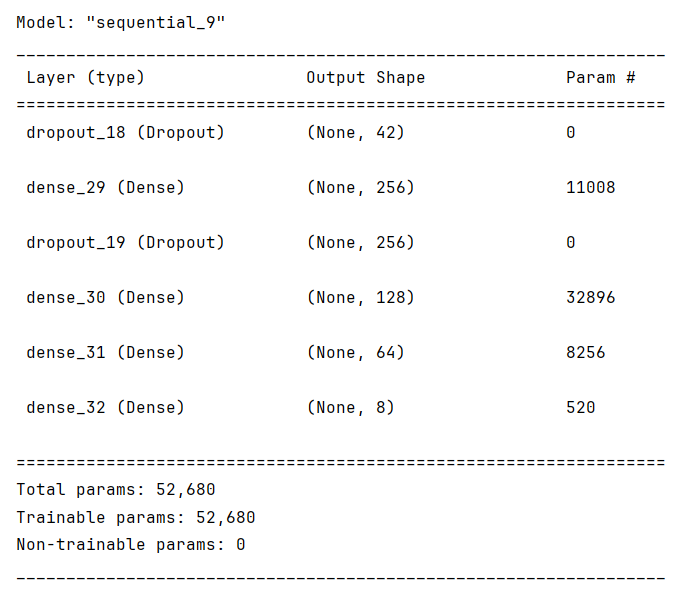
\includegraphics[width = 0.65\textwidth]{images/model_summ.png}
%	\caption{Configuration of the used feedforward neural network}
%	\label{fig:layers}
%\end{figure}
The following is a report on training our neural network with the data. We utilized a model, which comprises one input layer and one output layer, along with five hidden layers consisting of three dense layers and two dropout layers. The sequential application of dropout and dense layers with ReLU activation acts as a mechanism to prevent overfitting while allowing the model to make nonlinear mappings. The output layer of the neural network comprises neurons equivalent to the number of hand gestures it can recognize - 8. The configuration of the model is depicted in Figure \ref{fig:neural_network}. The was trained with a dataset split into training and testing sets (our particular model uses $75\%$ as the training data.) and was designed using the Adam optimizer, which is efficient and appropriate for training models with large data and parameters. The Sparse Categorical Crossentropy loss function was utilized to evaluate the loss between predicted and actual labels, while accuracy was used as the evaluation metric to determine how frequently the prediction matches the actual label. The training was halted by early stopping when the validation loss stopped to decrease and then converted into TensorFlow Lite to reduce its size. Initially, the training model was set to have only four hidden layers (2 dense layers). However, the training accuracy failed to exceed 90\%. Consequently, we updated the model to have five hidden layers (with 3 dense layers), without any other modifications and obtained satisfactory results. The training accuracy achieved was 99.62\%, and the calculated loss was 0.0309.





\section{Results}

To perform a quantitative analysis of the test dataset, we employed the  \text{classification report} and  \text{confusion matrix} libraries from scikit-learn. The \text{classification report} library produced an assessment report of our model with accuracy, precision, recall, and F1 score matrices. Additionally, the support matrix represents the model's real-time recognition performance.



\begin{table}[h]
	\centering
		\caption{Classification Report}
	\renewcommand{\arraystretch}{1.35} % Adjusts the row height
	\begin{tabular}{lcccc}
		\hline
		\textbf{Class}       & \textbf{Precision} & \textbf{Recall} & \textbf{F1-Score} & \textbf{Support} \\ \hline
		0                    & 0.99               & 1.00            & 0.99              & 622              \\
		1                    & 1.00               & 0.99            & 1.00              & 508              \\
		2                    & 1.00               & 0.98            & 0.99              & 556              \\
		3                    & 1.00               & 0.99            & 1.00              & 759              \\
		4                    & 1.00               & 1.00            & 1.00              & 621              \\
		5                    & 1.00               & 1.00            & 1.00              & 673              \\
		6                    & 0.98               & 1.00            & 0.99              & 666              \\
		7                    & 1.00               & 1.00            & 1.00              & 603              \\
		\textit{accuracy}    &                   & 0.99            &                 & 5008             \\
		\textit{macro avg}   & 1.00               & 0.99            & 0.99              & 5008             \\
		\textit{weighted avg} & 0.99               & 0.99            & 0.99              & 5008             \\ \hline
	\end{tabular}

	\label{tab:report}
\end{table}

Precision is the ratio of correctly predicted positive observations to the total predicted positive observations. 

The accuracy matrix calculates the number of correctly predicted labels by the model from the entire dataset (Eq.\ref{eq:accuracy}). 
The precision matrix measures the model's accuracy out of the predicted positives. It calculates the number of actual positives in the predicted positives and is an excellent measure to consider when the False Positive (FP) cost is high. Equation \ref{eq:precision} depicts the mathematical formula of the precision matrix.

The recall matrix measures the number of predictions our model correctly labels as positives. It is a measure considered when false negatives have high costs. The mathematical formulation of the recall matrix is Equation \ref{eq:recall}. 

The F1 score is calculated by combining both precision and recall, as shown in Equation \ref{eq:f1_score}. It is their harmonic mean.

Support is the number of samples in each class. 
The macro-average of precision, recall, and F1-score demonstrates the system's average performance across all classes, while the weighted average takes into account the class imbalance by weighting the metrics based on the number of samples in each class.\newline
Additionally, the loss value of $3.09\%$ (not shown) indicates how efficiently the model is minimizing its errors during training, while overall accuracy stands at $99.62\%$

The classification report of the implemented model in detail is shown in Figure \ref{fig:report}. 


\begin{equation}
	\text{accuracy} = \frac{TP + TN}{TP + TN + FP +FN}
	\label{eq:accuracy}
\end{equation}

\begin{equation}
	\text{precision} = \frac{TP}{TP + FP}
	\label{eq:precision}
\end{equation}
\begin{equation}
	\text{recall} = \frac{TP}{TP + FN}
	\label{eq:recall}
\end{equation}

\begin{equation}
	\text{F1 score} = \frac{2 P  R}{P+ R} 
	\label{eq:f1_score}
\end{equation}

In the equations (\ref{eq:accuracy}), (\ref{eq:precision}), (\ref{eq:recall}), and (\ref{eq:f1_score}), TP, TN, FP, and FN represent True Positive, True Negative, False Positive,
and False Negative, respectively.


The confusion matrix is a key performance metric used in machine learning, particularly in classification tasks. By utilizing the scikit-learn library in Python, one can create a confusion matrix. To conduct our experiment on predicting hand gestures, we obtained and pre-processed the necessary datasets. The confusion matrix was then utilized to evaluate the accuracy of our model, which is illustrated in Figure \ref{fig:confusion_matrix}. The x-axis represents predicted labels, while the y-axis represents actual labels.

Through the confusion matrix, we can pinpoint which gestures are being incorrectly recognized. For instance, we observed that gesture 2 was misinterpreted as gesture 6 a total of 11 times. We can further calculate the recall of gesture 2 utilizing Equation \ref{eq:recall2}:

\begin{equation}
	\text{recall(2)} = \frac{545}{545 + 11}
	\label{eq:recall2}
\end{equation}



The system's performance is satisfactory, with almost perfect precision, recall, and F1-score in most classes, as well as high accuracy and weighted average.

To find the model's performance from a loss validation standpoint, we can plot its progress throughout the epochs.

\begin{figure}[h]
	\centering
	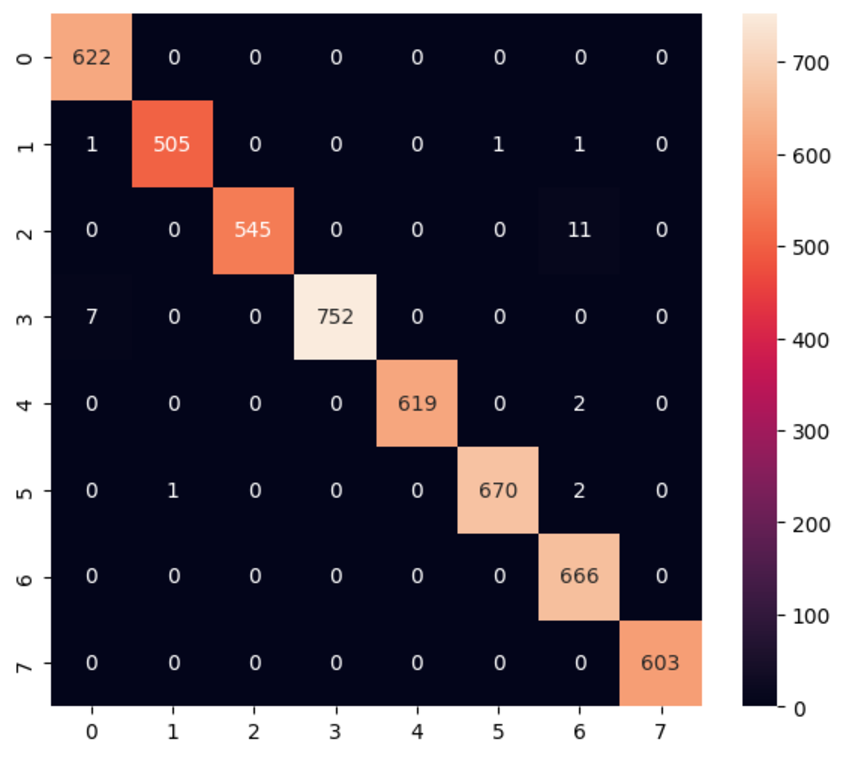
\includegraphics[width = 0.65\textwidth]{images/confusion_matrix.pdf}
	\caption{Confusion matrix of the model}
	\label{fig:confusion_matrix}
\end{figure}


\begin{figure}[h!]
	\centering
	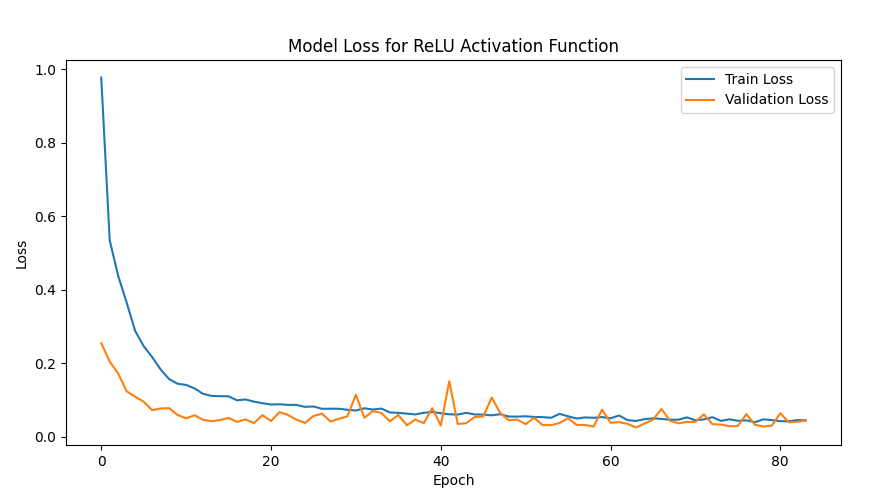
\includegraphics[width=\textwidth]{images/model_loss_relu.png}
	\caption{Training and validation loss curves for a neural network model utilizing the ReLU activation function.}
	\label{fig:model_loss_relu}
\end{figure}

The graph indicates a rapid decrease in loss in the initial epochs followed by a stable, low variance loss, demonstrating good model convergence without overfitting.

\subsection{Comparisons}
As we wanted to optimize our neural network, we conducted a comparison of the Stochastic Gradient Descent (SGD) and Adam optimizers. Figure \ref{fig:optimizers} shows that Adam achieves faster convergence, reduces loss swiftly, and maintains high accuracy, making it suitable for complex neural network training where time and resource optimization are as critical as model accuracy. On the other hand, SGD shows more gradual improvement and requires more epochs to reach comparable performance.

\begin{figure}[ht!]
	\centering
	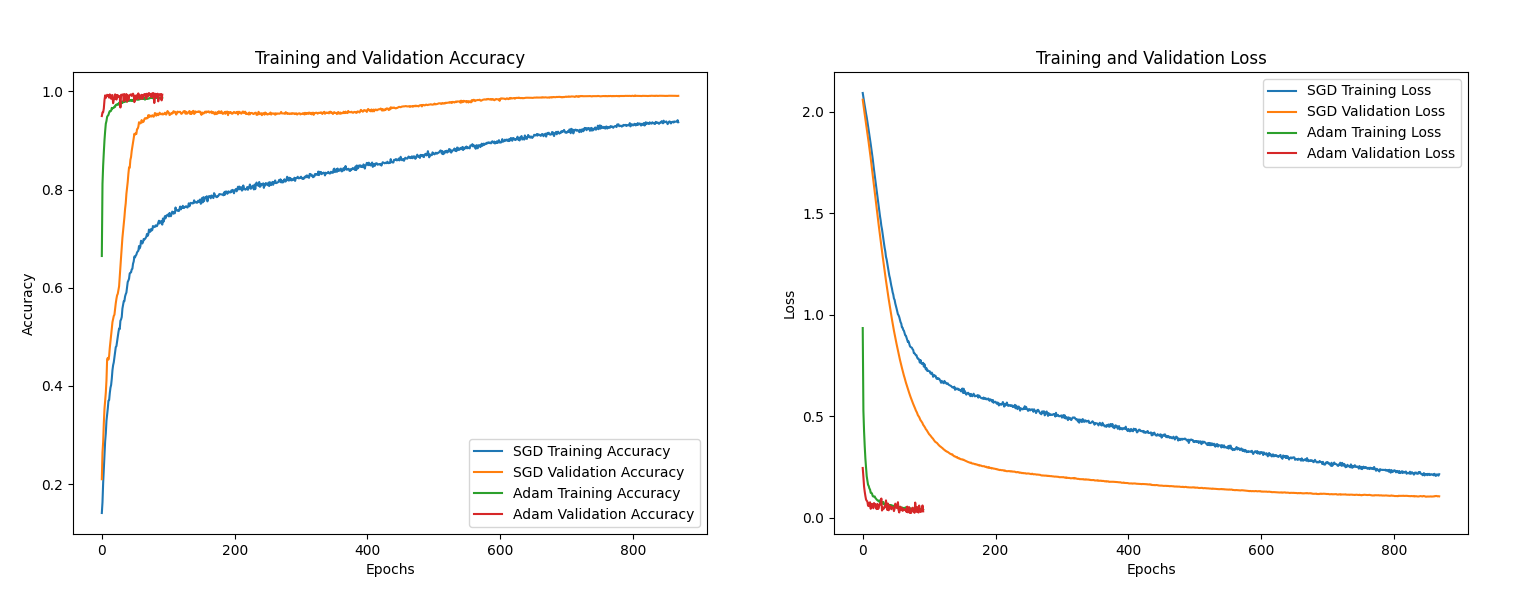
\includegraphics[width=\textwidth]{images/optimizers_comparison.png}
	\caption{Comparative analysis of different optimizers.}
	\label{fig:optimizers}
\end{figure}


We studied the impact of initial learning rates on Adam optimizer's performance. The initial learning rate has a significant effect on the convergence speed and training stability, as demonstrated in figure \ref{fig:learning_rates}.\newline
The model trained with a higher initial learning rate of $0.001$ (as used in our case) converges rapidly, as indicated by a swift decline in loss and a quick rise in accuracy. However, the models with lower initial rates of $0.0001$ and $1e^{-5}$ demonstrate a more gradual improvement, with the lowest rate showcasing the most stable but slowest progression.\newline
The initial learning rate serves as a multiplier to the adaptively computed rates and determines the starting point for adjustments.
\begin{figure}[ht!]
	\centering
	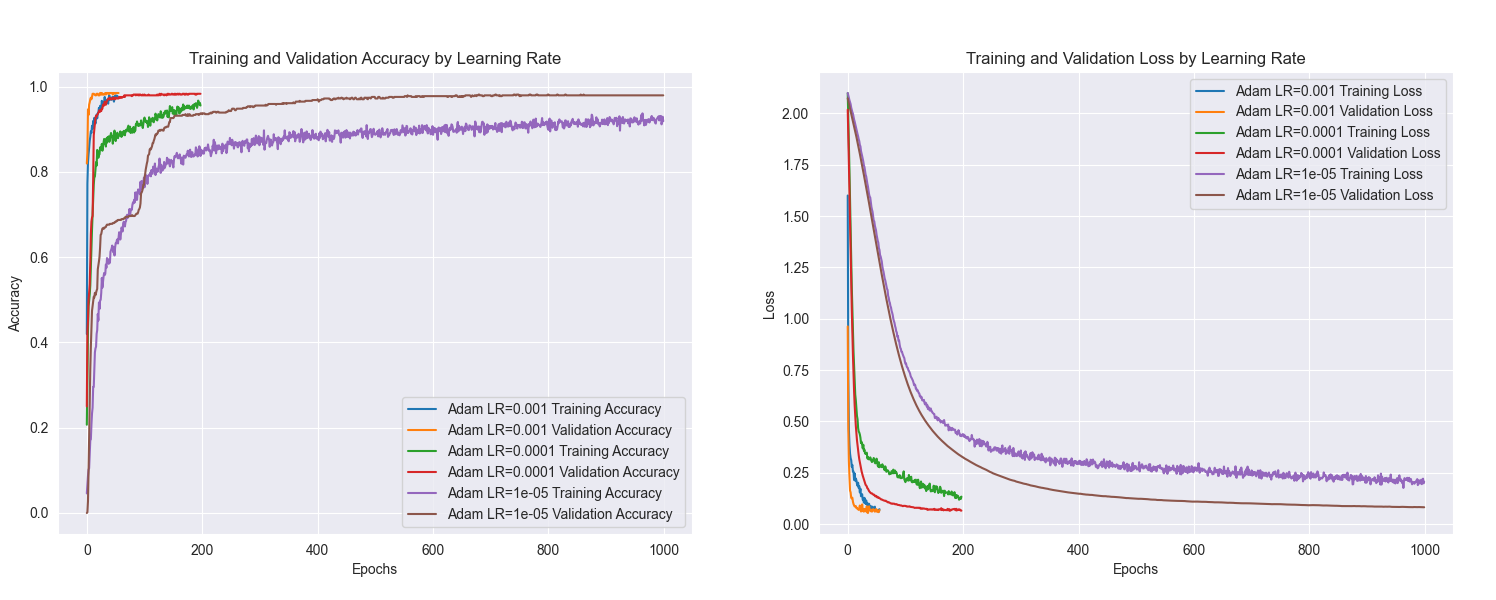
\includegraphics[width=\textwidth]{images/adam_learning_rates_comparison.png}
	\caption{Training and validation accuracy over epochs for different initial learning rates using the Adam optimizer.}
	\label{fig:learning_rates}
\end{figure}

We researched different batch sizes, ranging from 16 to 1024, to find the right one for our model. We found that smaller batch sizes, such as 16 and 64, decrease the loss quickly, but they are less stable and can make the convergence process more complicated. On the other hand, larger batch sizes, such as 512 and 1024, are more stable but converge slower, which means they may not use the training data as efficiently. The model's performance on each batch size is shown in figure \ref{fig:batch_sizes}

After considering all the options, we chose a batch size of 128. This size balances fast convergence with stable loss decrease and efficiently learns from the data. It is a good compromise between the noise observed in smaller batch sizes and the slow convergence observed in larger ones. The loss curve for a batch size of 128 is consistent, which means that our model has strong generalization performance. Therefore, we selected this batch size for our final model training.

\begin{figure}[h]
	\centering
	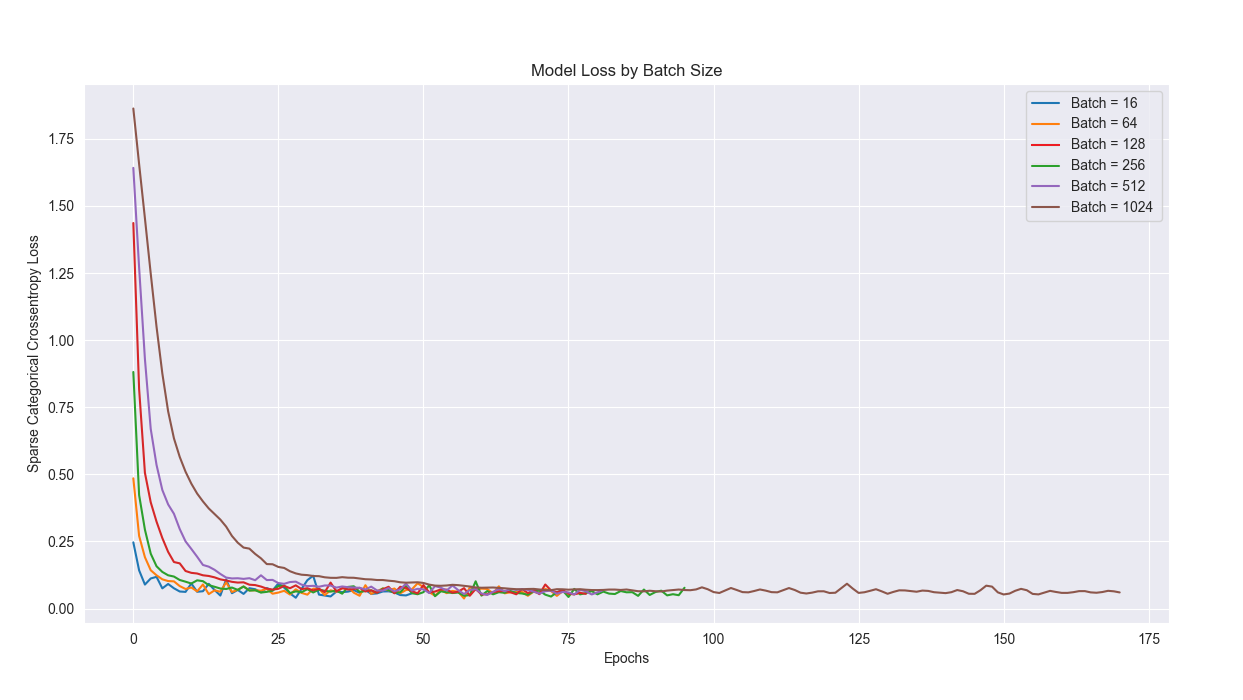
\includegraphics[width=\textwidth]{images/batch_sizes_comparison.png}
	\caption{The effect of batch size on model loss during training and validation.}
	\label{fig:batch_sizes}
\end{figure}

To sum up the importance of hyperparameters, we can look at the learning rate, as well as the number of epochs needed for the training. The comparisons of the impact of the hyperparameters on learning rate and epochs are shown in table \ref{tab:comparison_across_epochs}. It's important to note, that these exact models weren't used in our project, but the comparisons were done with our data.


\begin{table}[h!]
	\centering
		\caption{Comparison of optimizers, learning rates, and batch sizes across training epochs, with validation loss and epochs where learning plateaus.}
	\begin{tabular}{|c|c|c|c|}
		\hline
		\textbf{Parameter} & \textbf{Option} & \textbf{Validation Loss} & \textbf{Epochs} \\
		\hline
		\multirow{2}{*}{Optimizer} & SGD & 0.209 & 840 \\
		\cline{2-4}
		& Adam & 0.063 & 98 \\
		\hline
		\multirow{3}{*}{Learning Rate} & 0.001 & 0.112 & 73 \\
		\cline{2-4}
		& 0.0001 & 0.12 & 200 \\
		\cline{2-4}
		& 1e-5 & 0.18 & 1000 \\
		\hline
		\multirow{5}{*}{Batch Size} & 16 & 0.112 & 46 \\
		\cline{2-4}
		& 64 & 0.114 & 72 \\
		\cline{2-4}
		& 128 &  0.11& 77 \\
		\cline{2-4}
		& 256 &  0.12  & 94 \\
		\cline{2-4}
		& 512 & 0.113 & 80 \\
		\cline{2-4}
		& 1024 & 0.119 & 167 \\
		\hline
	\end{tabular}

	\label{tab:comparison_across_epochs}
\end{table}




Figure \ref{fig:epochs} shows the model's loss over 1000 epochs when using the ReLU activation function. The training loss decreases rapidly in the initial epochs, indicating the model is learning quickly and stabilizing. However, the validation loss fluctuates significantly throughout the training process, particularly in later epochs. This suggests that the model may be capturing noise or overfitting to the training data, continuing to learn beyond achieving minimal loss on the validation set.


\begin{figure}[ht!]
	\centering
	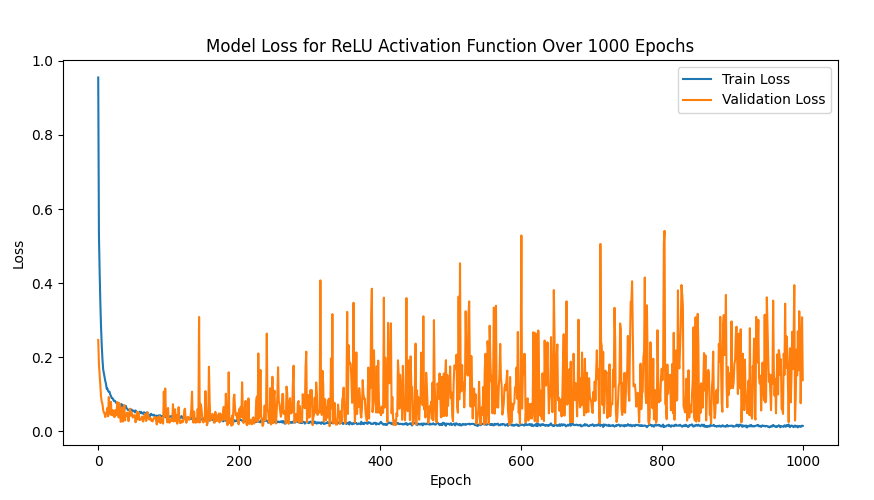
\includegraphics[width=\textwidth]{images/model_loss_over_1000_epochs.png}
	\caption{Model loss using the ReLU activation function plotted over 1000 epochs without early stopping.}
	\label{fig:epochs}
\end{figure}
The importance of implementing early stopping as a regularization technique (like in figure \ref{fig:model_loss_relu}) is underscored by this extended training. Without it, the model risks wasting computational resources and reducing its ability to generalize. The increasing divergence between training and validation loss after several hundred epochs reinforces the need for early stopping to halt training when the model ceases to improve in generalization to validation data.

\section{Drone Implementation}

The flow of this project is as follows: the drone flies off, and we process the image that is captured by the drone's camera. Using multiple models for detecting, classifying, and localizing features in the image, after detecting a face, our model returns a prediction of a gesture and the drone executes the corresponding command in real time. The logic of the process is presented in Figure \ref{fig:flowchart}


\begin{figure}
	\centering
	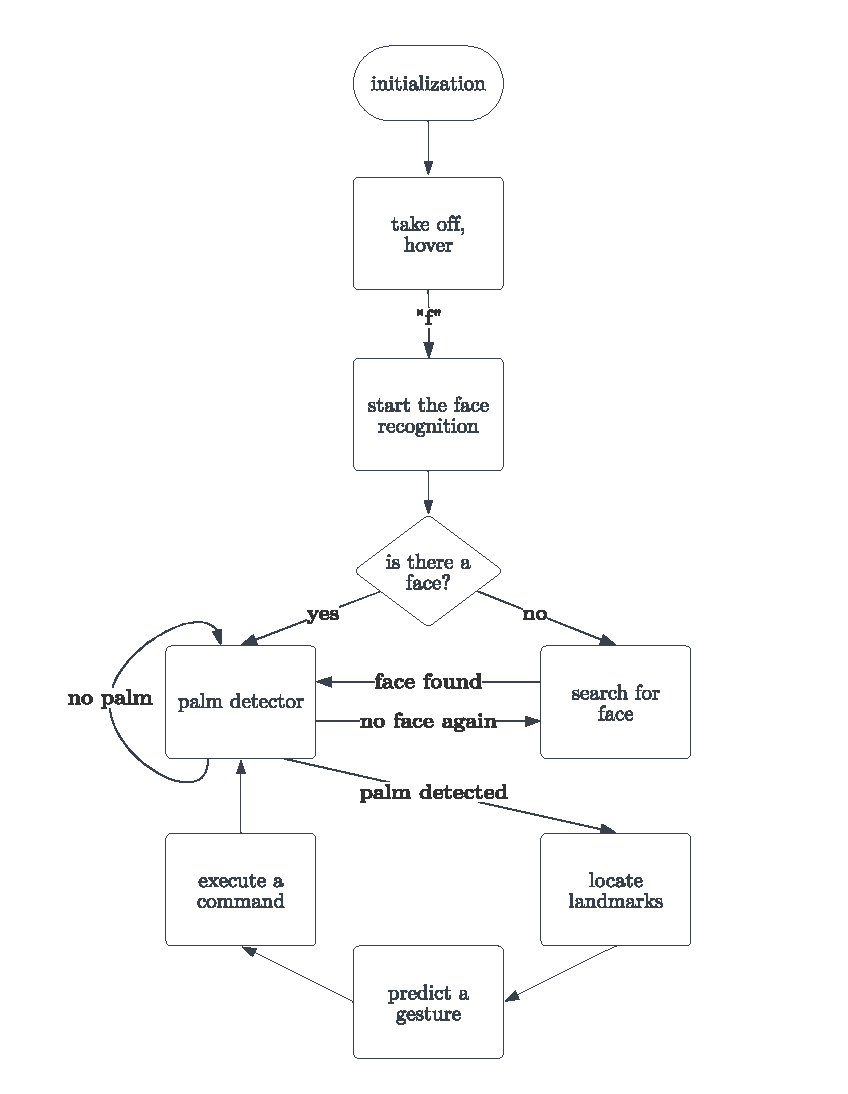
\includegraphics[width =1.1 \textwidth]{images/flowchart.pdf}
	\caption{Logic in the recognition process.}
	\label{fig:flowchart}
\end{figure}

The Tello drone is a compact quadcopter that boasts an advanced vision positioning system and a high-resolution (8 mp) onboard camera, designed to capture stunning aerial photographs and videos. It offers versatile operating options, allowing users to control it through a laptop computer or a smartphone. The drone connects to devices using Wi-Fi, which facilitates a stable and fast connection essential for real-time video streaming and responsive flight control. Additionally, it supports the 2.4 GHz frequency band for remote control, a widely used standard that ensures reliable communication over distances. The drone has other built-in functions like a range finder, barometer, LED, or vision system. It is fitted with a single accelerometer and 3-axis magnetometer (which can get the drone orientation), a pressure, and an IR-based altitude detector. The Tello drone is compatible with a dedicated smartphone application available on both Android and iOS platforms. This app unlocks several intuitive flight modes, easy-to-use controls, and creative functions.

The Tello library is a toolkit crafted to seamlessly integrate with Python. It's specifically designed for developers and hobbyists, offering easy access and control over the Tello drone's functionalities. With a comprehensive array of built-in functions, the library manages communication protocols with the drone, allowing for real-time transmission of control commands and reception of status updates. This ensures a smooth and responsive piloting experience.

Moreover, the Tello library efficiently handles state changes, adapting to various flight conditions and drone responses, such as battery levels, speed, and altitude. For example, if the drone is low on battery, it doesn't flip. This feature is essential for creating applications that require precise control and feedback from the drone, providing a foundation for developing flight patterns and maneuvers.

The library's event-driven control allows the execution of code in response to specific events, such as takeoff, landing, or moving in a direction with a designated speed.

\begin{figure}[h!]
	\centering
	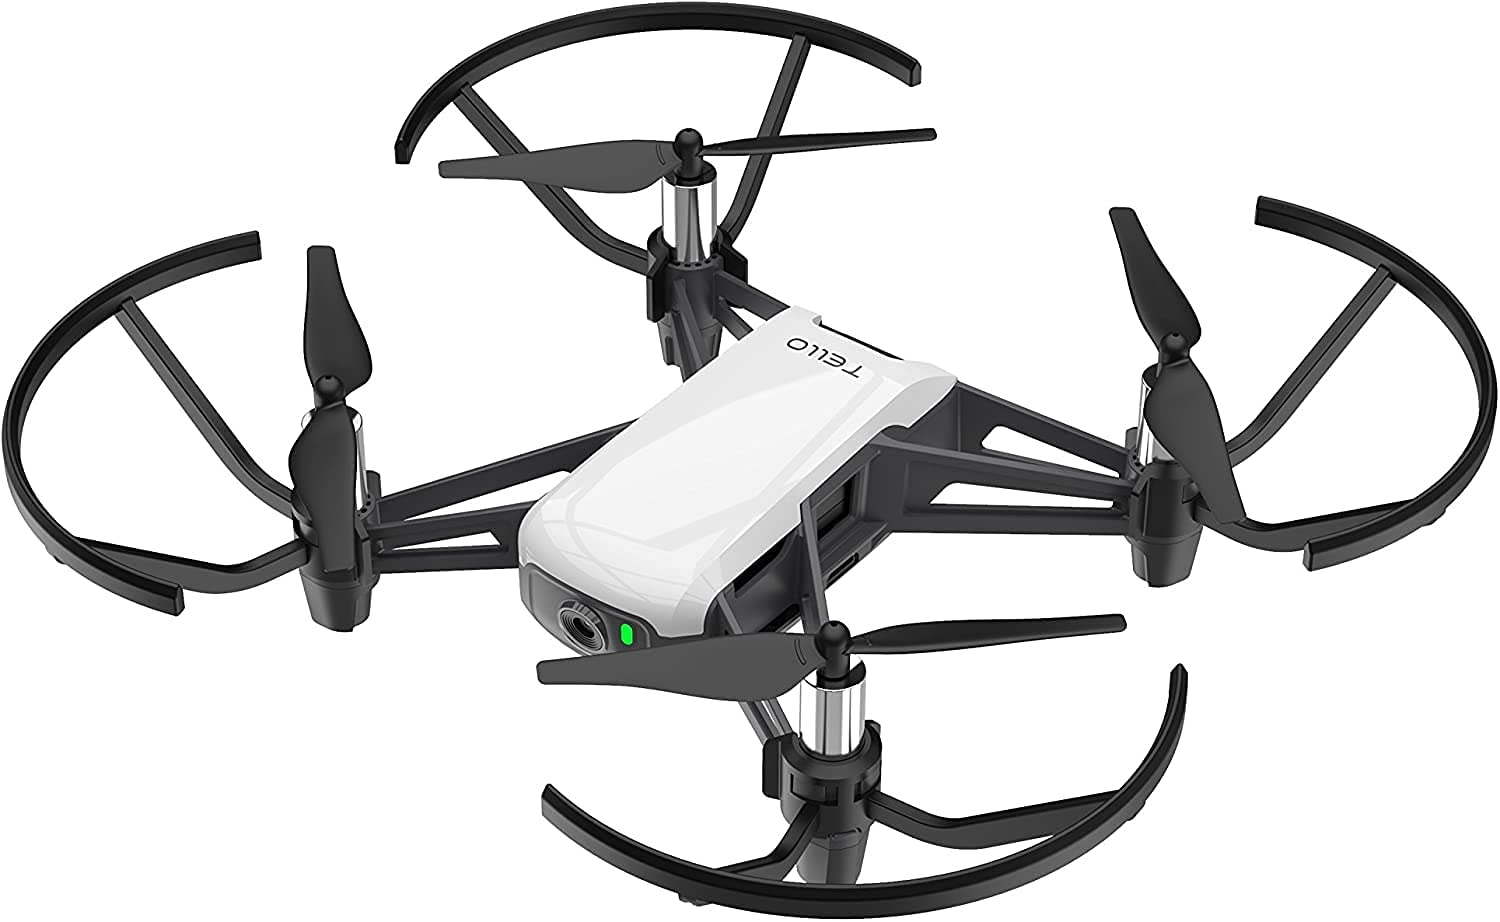
\includegraphics[width = 0.6\textwidth]{images/drone.jpg}
	\caption{Drone used in this project.}
	\label{fig:tello}
\end{figure}

To operate a drone, we can use specific hand gestures as commands. This technique is chosen due to its ease of use and intuitive nature. Additionally, Tello provides a Python API that streamlines the process of drone operation. This API eliminates the need for direct manipulation of the motor hardware, allowing us to focus on perfecting our hand gestures and achieving more precise control of the drone. For this to work, we just set each gesture ID to a command.



Table \ref{tab:gesture_commands} lists the commands used in our project, which were assigned to the labels of our gestures. The gestures we utilized can be found in Figure \ref{fig:all_gestures}.

\begin{table}[ht]
	\centering
		\caption{Gesture commands for drone control}
	\begin{tabular}{ll}
		\toprule
		Gesture Label & Command \\
		\midrule
		0 - Palm& Move along the y-axis (forward velocity) \\
		1 - Fist& Move along -y-axis (backward velocity) \\
		2 - Rock& Flip forward (upward velocity) \\
		3 - OK & Take-off or land (depending on whether in flight or landed) \\
		4 - Peace& Takes a picture (saves in png) \\
		5 - Like& Rotate 360$^\circ$ \\
		6 - Up& Move up (ascending velocity) \\
		7 - Down & Move down (descending velocity)\\
		\bottomrule
	\end{tabular}

	\label{tab:gesture_commands}
\end{table}

Our program prompts the Tello drone to begin executing commands after a key press and identifies a gesture every 5 seconds. This allows for the comfortable execution of a command before recognizing the next one. After tweaking speeds and sleep times, the Tello drone executed the received commands rapidly and consistently.

\begin{figure}[ht]
	\centering
	\begin{minipage}{0.5\textwidth}
		\centering
		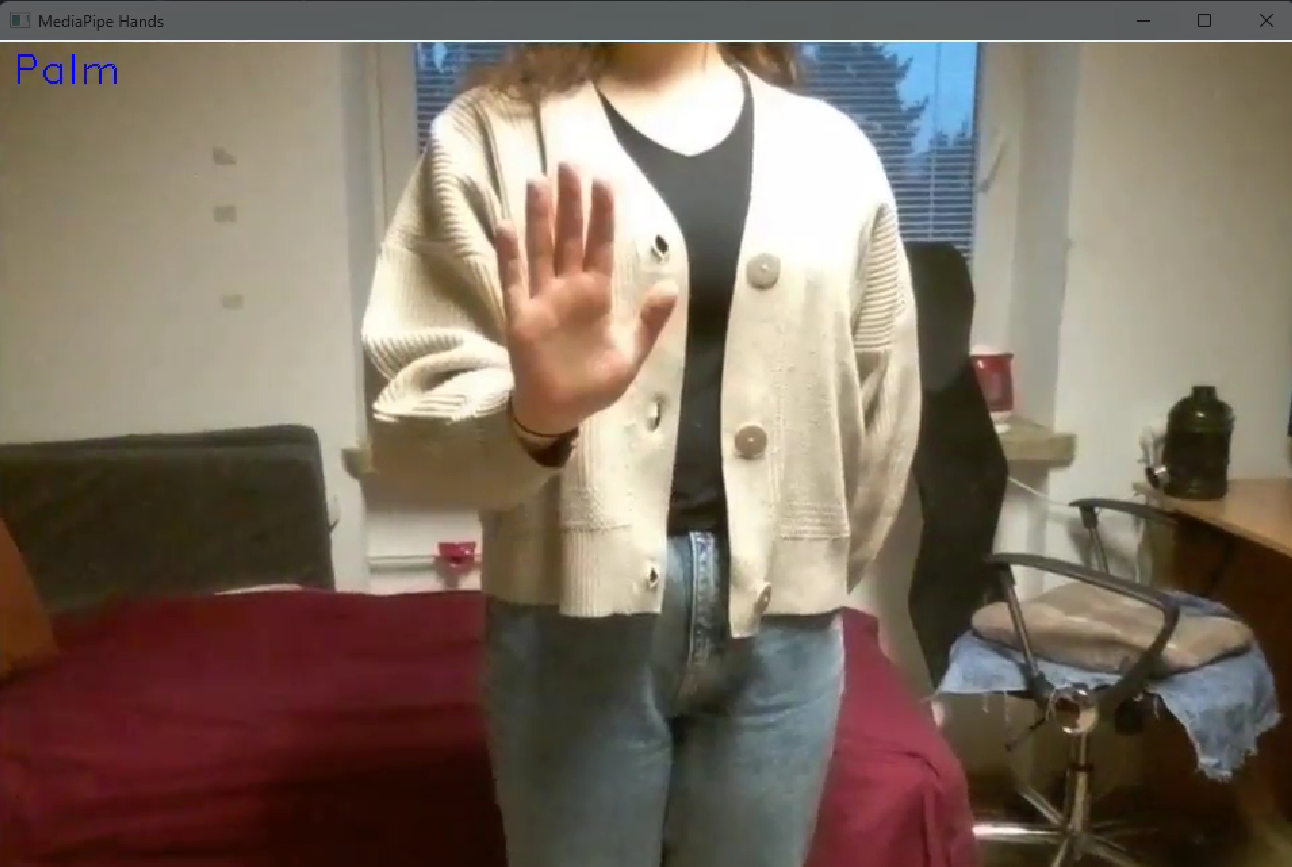
\includegraphics[width=0.85\textwidth]{images/palm_drone.png}
		%   \caption{Landmarks for pose estimation model by MediaPipe}
	\end{minipage}% <-- This percentage sign denotes the end of a minipage
	\begin{minipage}{0.5\textwidth}
		\centering
		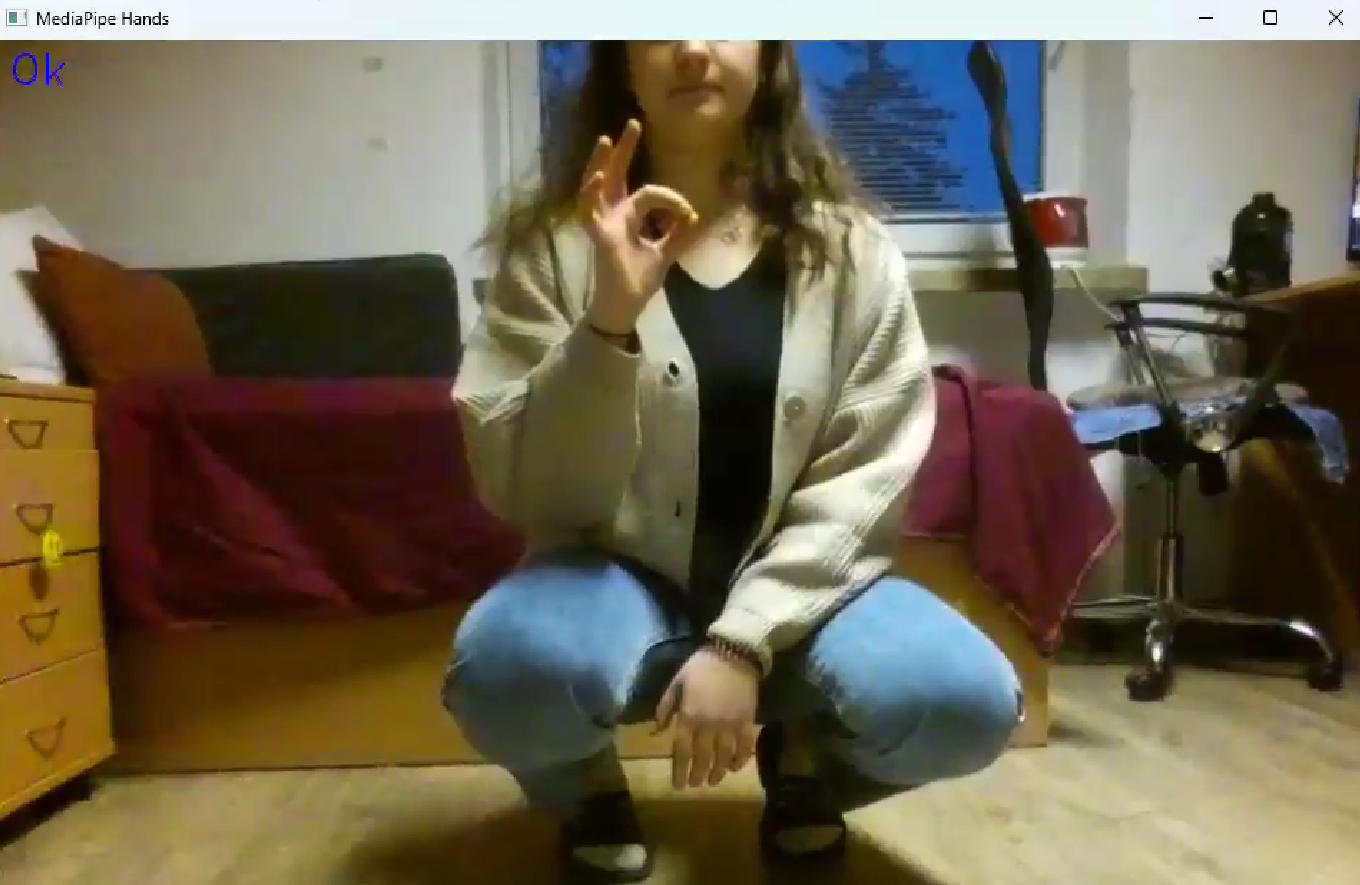
\includegraphics[width=0.85\textwidth]{images/ok_drone.png}
		%   \caption{U-Net segmentation on an image from Oxford-IIIT Pet Dataset (Parkhi et al, 2012).}
	\end{minipage}
	\caption{Gesture recognition shots from the drone camera.}
	\label{fig:drone_detections} % This label can now be used to reference both images together
\end{figure}

In Figure \ref{fig:drone_detections} we can observe the various gestures identified by the drone's camera. Upon recognizing the 'Palm' gesture, the drone would proceed to move backward. In the subsequent image, we see the drone on the ground, and upon recognizing the 'Ok' gesture, it would take off to a predetermined altitude.
In addition, if we are not recognizing any gesture, the drone is ready to land on the palm. Because the drone can execute most of the commands only while flying, it takes off at the start of the program. It can also take off with gesture 4, so the program doesn't have to be reset.


\section{Future Work}
Moving forward with our work, there is ample room for the expansion of the project. We have developed a good gesture classifier that can be utilized for other applications besides drones, such as smart home control, sign language translation, multimedia control, or security systems. For example, a previous study \cite{doi:10.1080/08839514.2023.2176607} used a gesture recognizer and ESP8266 microcontroller to control home appliances using gestures to adjust a simple LED light, turning it on/off, setting its brightness and color.

If we decide to implement face recognition, there are many popular face recognition systems available that we can use. Facial recognition systems are widely used in modern life, making authentication processes easier without the need for passwords or physical IDs. Some examples of algorithms used for face recognition include Eigenfaces \cite{CARIKCI2012118}, Local Binary Patterns Histograms (LBPH) \cite{inproceedings}, Fisherfaces, Scale-Invariant Feature Transform (SIFT) \cite{articlefr}, and Speed Up Robust Features (SURF) \cite{10.1007/11744023_32}. The Haar Cascade classifier by Paul Viola and Michael Jones \cite{inproceedings} is the first choice for face detection alone.


\begin{figure}[h]
	\centering
	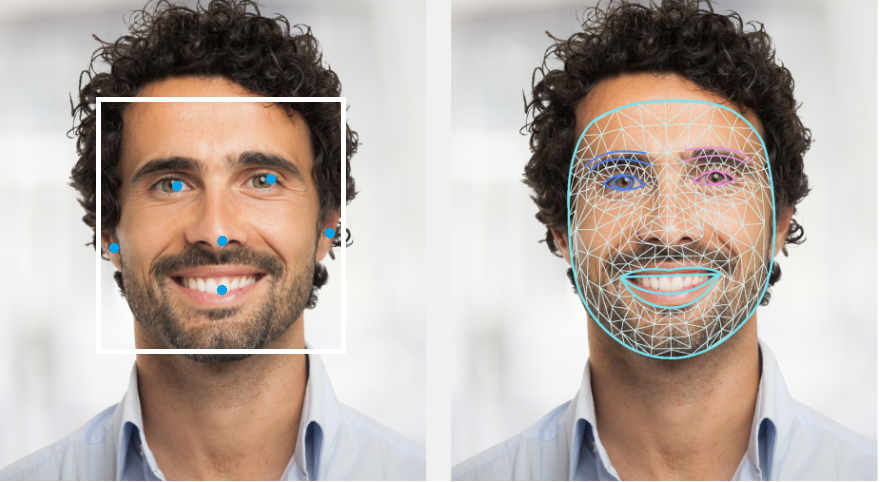
\includegraphics[width=0.8\textwidth]{images/face_landmark.png}
	\caption{Outputs of FaceBlaze and Face Landmark model.}
	\label{fig:face_landmark}
\end{figure}

\par~
\newline



Since we are using Mediapipe, we opted to use their Face Landmark model to extract 478 3-dimensional face landmarks. This model works in conjunction with the BlazeFace detection model and the Face mesh model. Figure \ref{fig:face_landmark} shows the difference in outputs of each model. We applied these models in a similar way as we did with the hand models, using spatial positions of the landmarks. Firstly, we collected our data, labeling each capture of the face with a label. Then, we trained a simple KNN model to predict the person in the picture. However, since our database is not large (as we only tested with two people, and the prediction is real-time), it is difficult to conclude whether the model is sufficient for higher usage. Nevertheless, it demonstrates an alternative way for face recognition using only Mediapipe models. The face recognition model is saved in our repository \cite{touchlessdronecontrol}.





% conclusions
\chapter{Conclusions}
The aim of this thesis was to design and develop a reliable system that classifies hand gestures for controlling a drone through an embedded camera system. This was achieved by integrating machine learning models for real-time image processing. MediaPipe, an open-source framework, was utilized for hand tracking, while TensorFlow, an open-source machine learning framework, was used for developing the model. To classify gestures efficiently, a neural network was designed based on deep learning research. The model was designed to handle diverse hand orientations and lighting conditions encountered during drone operation. The backbone of this achievement was the fact, that the model wasn't trained on just images processed with classical methods, but rather extracted features were represent 21 landmarks on each hand.

To evaluate the efficiency of the prediction model, it was empirically tested, and an accuracy of 99.62\% was achieved on the testing set. The model's ability to generalize well to new, unseen data was a critical requirement for real-world applications, and this was achieved through a meticulously designed classification report that yielded high precision, recall, and F1-scores across all classes. The model's architecture is based on deep learning research and employs dropout layers and dense networks with ReLU activations.

The model's ability to differentiate between nuanced hand positions effectively was demonstrated, ensuring reliable drone navigation commands. The minimal number of misclassifications is indicative of the model's capacity to differentiate between nuanced hand positions effectively. A quantitative analysis using a confusion matrix was done to discern the model's ability to differentiate between similar gestures with a high degree of accuracy.

The model was implemented in TensorFlow Lite, which showcased an effective translation of computational efficiency and performance into an embedded system context, such as the Tello drone used in this study. This implementation demonstrates the practical feasibility of applying advanced machine learning algorithms in resource-constrained environments, which is a key consideration in the development of autonomous systems.

In conclusion, the thesis aimed to design, develop, and implement a machine learning system that provides accurate, efficient, and reliable gesture-based control of a drone. Through extensive testing, the practical applications of this system were validated, and its adaptability across a range of gestures and operational scenarios was confirmed. This achievement lays the groundwork for future advancements in touchless drone control interfaces and opens new avenues for exploration in the field of human-computer interaction.
\clearpage

% Appendices (Prílohy) comment by "%" if not neccesary
\appendix
 \chapter{Resumé}
 \label{ch:resume}
Táto bakalárska práca sa zaoberá teoretickými a praktickými aspektmi strojového učenia a jeho aplikáciami v počítačovom videní, neurónových sieťach a rozpoznávaní gest. V teoretickej časti sa zameriava na preskúmanie rôznych techník učenia, ako je učenie s učiteľom, či bez učiteľa, no najmä metódami počítačového videnia, ako sú klasifikácia, detekcia a segmentácia.\newline
 Počítačové videnie využíva klasifikáciu na rozpoznanie vlastností objektov, z ktorých potom určuje do ktorých kategórií tieto objekty patria. Pre samotnú klasifikáciu platí všeobecný postup: predspracovanie obrazu $\to$ extrakcia čŕt $\to$ klasifikácia objektov. Klasifikáciu možno taktiež rozdeliť na binárnu, kde výstupom je jedna z dvoch možností, multi-class, kde výstup je výber z viac ako dvoch možností, klasifikáciu viacerých značiek (multilabel), kde výstupu možno priradiť viac ako jednu možnosť alebo hierarchickú klasifikáciu, kedy sa triedy radia do hierarchickej štruktúry na základe podobnosti. Triedy nižších úrovní sú konkrétnejšie a detailnejšie ako triedy vyšších úrovní. Pri detekcii objektov, platí že jej výstupom sú ohraničujúce obdĺžniky, ako aj trieda do ktorej objekt patrí. Detekcii veľmi podobnou úlohou je segmentácia, kde princípom je nájdenie a oddelenie jednotlivých objektov od pozadia s presnosťou na pixely.\newline
Ďalej sa v teoretickej časti venujeme neurónovým sieťam. Neurónová sieť je sieť pospájanýh neurónov, medzi ktorými sa posúvajú informácie.	Pri doprednej sieti sa informácia posúva vpred, od vstupných neurónov k výstupným, a to cez skryté vrstvy neurónov. Vstupnú vrstvu tvoria priamo dáta vlastností, zatiaľ čo údaje získané z výstupnej vrstvy slúžia ako základ pre klasifikáciu vstupných dát. Neurón má niekoľko vstupov  ($x_1, x_2, ..., x_n$) a jeden výstup $\hat{y}$, pričom každý vstup má svoju „váhu“, teda dopredu dané číslo, ktoré vyjadruje významnosť jednotlivých vstupov. Neurón vezme vážený súčet vstupov spolu s vychýlením (bias) a aplikuje naňho aktivačnú funkciu. Aktivačné funkcie sú základným prvkom neurónových sietí a poskytujú im nelinearitu potrebnú pre modelovanie zložitých vzorcov. Aktivačná funkcia môže byť rôzna, ako napríklad sigmoid, softmax alebo ReLU (Rectified Linear Unit). Voľba aktivačnej funkcie výrazne ovplyvňuje rýchlosť, s akou algoritmus učenia dosahuje konvergenciu. Jej správny výber je podmienený štruktúrou a charakteristikami dát a účelom modelu. Aktivačné funkcie predstavujú matematické vzorce, ktoré určujú výstupy modelu. \newline
Tréning neurónovej siete môže byť opísaný ako iteračný proces aktualizovania parametrov siete. Cieľom tréningu je nájsť vektor váh, ktorý minimalizuje vybranú chybovú funkciu. Chybová funkcia predstavuje mieru správnosti či chybovosti. Postup trénovania siete možno zhrnúť v štyroch krokoch: 
\begin{enumerate}[label=\arabic*.]
	\item Po inicializácii náhodných váh začne popredné šírenie informácií, postupné vyhodnotenie výstupov vo všetkých vrstvách, až do poslednej. 
	\item Výpočet chyby. Chybu určuje chybová funkcia vzhľadom na skutočnú výslednú hodnotu. Príkladom chybovej funkcie je stredná kvadratická chyba (MSE) alebo krížová entropia.
	\item Algoritmus spätného šírenia. V tomto kroku sa minimalizuje chybová funkcia pomocou optimalizátorov (zostup gradientu, stochastický zostup gradiantu, či Adam).
	  Pomocou gradientu chybovej funkcie sa určuje, ako veľmi zmena každého parametra ovplyvní celkovú chybu.
	\item Aktualizácia váh. Po získaní smeru minimalizácie stratovej funkcie pomocou gradientu, je pre aktualizovanie váh potrebná aj dĺžka kroku. Pre neurónové siete sa pre dĺžku kroku používa označenie rýchlosť učenia. Nová váha je potom určená na základe získaného gradientu a rýchlosti učenia.
\end{enumerate}

Okrem rýchlosti učenia poznáme ďalšie nastavenia neurónových sietí, tzv. hyperparametre, ako veľkosť dávky (batch size), ktorý definuje počet vzoriek dát, na ktorých sa sieť učí v jednej iterácii trénovacieho cyklu, známom ako epocha. Počet epoch určuje, koľkokrát sieť uvidí celú trénovaciu sadu.\newline
Pri trénovaní sietí sa taktiež často implementujú techniky ako dropout alebo skoré zastavenie, ktorých nastavenie môžu priaznivo vplývať na generalizáciu, čas potrebný na tréning a môže zabrániť učeniu na "zašumenom" datasete. \newline
Teoretická  časť  																																
práce taktiež zahŕňa úvod do problematiky rozoznávanie gest a ukáže alternatívu rozoznávania gest počítačovým videním, a to pomocou dátovej rukavice Cyberglove II. \newline
V praktickej časti vysvetlíme implementáciu systému rozpoznávania gest s využitím frameworku MediaPipe. Priblížime si náš model neurónovej siete a výsledky jeho učenia. Kapitola ďalej obsahuje porovnanie rôznych optimalizačných algoritmov strojového učenia, ktoré poukazujú na ich vplyv na dynamiku a výsledky tréningu modelu. Nakoniec si priblížime využitie modelu pre ovládanie dronu Tello prostredníctvom rozpoznaných gest.\newline
 MediaPipe je framework pre vytváranie reťazcov pre spracovanie údajov v oblasti strojového učenia. Pre sledovanie rúk sme využili 2 spolupracujúce modely od MediaPipe: detektor dlane a model pre získanie orientačných bodov v dlani. Výstupom týchto modelov je súbor normalizovaných súradníc x, y pre každý tento orientačný bod na ruke. V projekte sme taktiež využili model MediaPipe Face, ktorého výstupom sme získali ohraničujúci obdĺžnik okolo tváre.\newline
Pre skúmanie vytvoreného modelu a jeho vyhodnotenie, je potrebné najskôr predstaviť priebeh projektu: dron vzlietne a náš program pomocou počítačového videnia spracováva obraz zachytený jeho kamerou. Pomocou viacero modelov, vrátane nami vytvoreného modelu na rozoznávanie gest, ako aj modelu na rozoznanie tváre v obraze, začneme rozoznávať tvár. Po rozoznaní tváre začneme rozoznávať gestá, zatiaľ čo opakovane kontrolujeme prítomnosť tváre. Dané gesto je prevedené na príkaz, ktorý dron vykoná.\newline
Model, ktorý sme použili na rozpoznávanie gest, je plne prepojená dopredná neurónová sieť. Model je prispôsobený na prácu s údajmi generovanými pomocou KeyPointClassifier, ktorý spracováva údaje modelov MediaPipe Hands. Model bol trénovaný na datasete rozdelenom na trénovacie a testovacie množiny (v našom prípade 75\% trénovacích údajov) a bol trénovaný s použitím optimalizátora Adam. 
Dataset s gestami sme zbierali pomocou osobitného programu, v ktorom sme dáta značili stlačením klávesy 0-7, v ktorom taktiež hral úlohu KeyPointClassifier. Konečný dataset obsahoval vyše 5000 vzoriek a bol uložený vo formáte csv, kde pri každom geste bol súbor súradníc x,y pre každý záchytný bod ruky. Výsledky modelu sa kvantitatívne analyzujú pomocou knižníc na vytváranie klasifikačných výsledkov a pravdivostnej matice. Celková presnosť modelu dosiahla 99,62\%. Náš dataset sme trénovali pod rôznymi nastaveniami hyperparametrov, ako aj pomocou optimalizátora stochastického gradientného zostupu. Tieto výsledky sme nakoniec porovnali. \newline
Pri časti, keď sme pracovali s dronom, je potrebné vyzdvihnúť Tello dron od spoločnosti RYZE Tech, ktorý je ideálny pre našu prácu, kvôli jeho dobrej kamere, váhe a cene. Využitím Tello knižnice sme najskôr testovali dané príkazy pomocou kláves. Po prevedení potrebných úprav pre hladšie pohyby dronu, sme implementovali náš model.\newline
Na záver sme preskúmali možné pokračovania práce, ako je autorizácia pomocou tváre pomocou modelu Face Landmark pred začatím rozpoznávania gest.




% Resumé v slovenčine, sa píše v prípade, že záverečná práca ja napísaná v 
% anglickom jazyku. Rozsah resumé tvorí 5-10\% rozsahu diplomovej práce.

%----------------------------------------------------------------%
%  The Backmatter !! Do NOT change the structure!!               %
%----------------------------------------------------------------%

\nocite{*}
% Bibliography to TOC
% do not remove
\backmatter

\providebibliography
\bibliography{bibfile}

%----------------------------------------------------------------%
%   The end of the document                                      %
%----------------------------------------------------------------%
\end{document}
